%% RespSalience -- Supplementary Material (standalone; compiles by itself with pdfLaTeX)
%% Proposed model: RespSalience. Regression baseline: PRISM-Breath.
%% No bibliography needed; references to the main paper are by name.
\documentclass[journal]{IEEEtran}
\usepackage[cmex10]{amsmath}
\usepackage{array}
\usepackage{booktabs}
\usepackage{amssymb}
\usepackage{multirow}
\usepackage{graphicx}

\renewcommand{\thetable}{S\Roman{table}}
\renewcommand{\thesection}{S\arabic{section}}
\renewcommand{\thefigure}{S\arabic{figure}}

\begin{document}

\title{Supplementary Material\\ Beyond Respiratory-Rate Regression: Decision-Aware Modeling for
Contactless Pediatric Tachypnea Screening}
\author{Imran~Rimon}
\markboth{IEEE Journal of Biomedical and Health Informatics -- Supplementary}{}
\maketitle

\noindent This document supplements the main paper with (i) complete per-fold results for
PRISM-Breath and four of the five published extractors (PhysFormer is omitted here: its stored predictions carry no tachypnea probability, so it cannot enter the per-fold AUROC table), (ii) an extended design-variant table, and (iii) the
full training and inference hyperparameters. All numbers are computed from the same subject-disjoint
five-fold cross-validation prediction files used in the main paper; every subject is tested exactly once.

\section{Per-Fold Results}
Tables~\ref{tab:s1}--\ref{tab:s3} give the fold-level breakdown behind the pooled numbers in the main
paper. Folds are subject-disjoint; the decision for sensitivity/specificity applies the WHO age-band
threshold to the predicted rate ($\hat r \ge \tau_{\text{age}}$). Fold~0 is consistently the hardest for
every method (lowest AUROC, highest MAE), indicating a genuinely difficult subject subset rather than
model instability---PRISM's advantage holds even there ($0.812$ vs.\ $0.613$--$0.681$).

\begin{table}[!t]
\caption{PRISM-Breath per-fold clinical performance (subject-level).}
\label{tab:s1}\centering\small
\setlength{\tabcolsep}{4pt}
\begin{tabular}{@{}lcccccc@{}}\toprule
Fold & $n$ & pos & RR-MAE & Sens & Spec & AUROC\\\midrule
Fold 0 & 67 & 20 & 7.84 & 0.65 & 0.94 & 0.766 \\
Fold 1 & 67 & 19 & 5.63 & 0.53 & 0.90 & 0.808 \\
Fold 2 & 66 & 15 & 5.67 & 0.67 & 0.98 & 0.939 \\
Fold 3 & 66 & 16 & 6.17 & 0.25 & 0.94 & 0.845 \\
Fold 4 & 66 & 14 & 5.79 & 0.64 & 0.87 & 0.857 \\
\midrule
\textbf{Pooled} & 332 & 84 & 6.22 & 0.55 & 0.92 & 0.827 \\
\textbf{Mean$\pm$SD} & --- & --- & $6.22{\pm}0.93$ & --- & --- & $0.843{\pm}0.064$ \\
\bottomrule
\end{tabular}
\end{table}

\begin{table*}[!t]
\caption{Per-fold tachypnea AUROC (298 matched subjects for baselines; PhysFormer omitted, see text).}
\label{tab:s2}\centering\small
\begin{tabular}{@{}lccccc@{}}\toprule
Method & Fold 0 & Fold 1 & Fold 2 & Fold 3 & Fold 4\\\midrule
\textbf{PRISM-Breath} & \textbf{0.766} & \textbf{0.808} & \textbf{0.939} & \textbf{0.845} & \textbf{0.857} \\
EfficientPhys & 0.681 & 0.750 & 0.770 & 0.821 & 0.750 \\
DeepPhys & 0.675 & 0.793 & 0.808 & 0.823 & 0.715 \\
TS-CAN & 0.626 & 0.814 & 0.730 & 0.707 & 0.758 \\
VIRENet & 0.613 & 0.807 & 0.933 & 0.765 & 0.680 \\
\bottomrule
\end{tabular}
\end{table*}

\begin{table}[!t]
\caption{Per-fold RR mean-absolute-error (breaths/min); PhysFormer omitted, see text.}
\label{tab:s3}\centering\small
\begin{tabular}{@{}lccccc@{}}\toprule
Method & Fold 0 & Fold 1 & Fold 2 & Fold 3 & Fold 4\\\midrule
PRISM-Breath & 7.84 & 5.63 & 5.67 & 6.17 & 5.79 \\
EfficientPhys & 7.66 & 5.38 & 5.82 & 6.14 & 5.51 \\
DeepPhys & 7.54 & 4.17 & 5.46 & 5.74 & 5.12 \\
TS-CAN & 8.36 & 4.26 & 5.81 & 6.98 & 5.34 \\
VIRENet & 8.53 & 4.13 & 4.11 & 6.89 & 5.94 \\
\bottomrule
\end{tabular}
\end{table}

\noindent\textit{Note on the MAE/AUROC dissociation.} In Table~\ref{tab:s3} the baselines are competitive
on per-fold MAE (indeed VIRENet is best on Folds~1--2), yet in Table~\ref{tab:s2} PRISM leads on AUROC in
every fold. This fold-level view reinforces the main-paper thesis: lower regression error does not imply
better tachypnea discrimination.

\section{Extended Design-Variant Ablation}
Table~\ref{tab:s4} lists additional variants beyond the main-paper ablation, evaluated under the identical
pooled five-fold protocol on all 332 subjects. Frequency-forward fusion, heteroscedastic/synthetic
adapters, and a compact AirFlow head neither help nor hurt materially; the hand-crafted optical-flow
channel (``v3'') is competitive in-domain but collapses out-of-domain (main paper, Table~VI). Among
sequence backbones, neither a Mamba-style state-space fusion nor a CliffPhys-style backbone differs
significantly from PRISM's reliability-weighted fusion---another instance of the architecture mattering
less than the decision rule.

\begin{table*}[!t]
\caption{Extended design variants (pooled five-fold). DeLong $p$ is paired against full PRISM
(AUROC $0.827$) on the subject intersection; ``n.s.'' $=$ not significant. Two variants were trained on
the 297-subject learned-flow signal set and are marked accordingly. Note that two variants
\emph{exceed} the full model, consistent with the ablation finding that no component is individually
load-bearing.}
\label{tab:s4}\centering\small
\begin{tabular}{@{}lcccc@{}}\toprule
Variant & $n$ & RR-MAE & AUROC & DeLong $p$ vs.\ PRISM\\\midrule
PRISM-Breath (full) & 332 & 6.22 & 0.827 & --- \\
Flow-only (depth/audio off) & 332 & 6.15 & \textbf{0.890} & $3.0{\times}10^{-4}$ \\
Frequency-forward fusion & 297 & 6.38 & 0.870 & $0.033$ \\
Heteroscedastic $+$ synthetic & 297 & 6.72 & 0.855 & $0.148$ (n.s.) \\
Hand-crafted flow (v3) & 332 & 6.20 & 0.853 & $0.426$ (n.s.) \\
AirFlow-compact head & 332 & 6.54 & 0.842 & $0.447$ (n.s.) \\\midrule
Mamba-fusion backbone & 332 & 7.55 & 0.809 & $0.419$ (n.s.) \\
CliffPhys-style backbone & 332 & 6.53 & 0.850 & $0.280$ (n.s.) \\\bottomrule
\end{tabular}
\end{table*}

\section{Hyperparameters}
Tables~\ref{tab:s5}--\ref{tab:s6} report the exact settings used. Both models are compact: the
PRISM-Breath baseline uses $d_{\text{model}}=64$ and sequence length $300$, and RespSalience is a
four-block one-dimensional convolutional encoder ($32/64/128/128$ channels) followed by a linear
salience head over $169$ rate bins. Headline operating points for RespSalience are averaged over three
training seeds ($0,1,2$).

\begin{table}[!t]
\caption{PRISM-Breath model and supervised-training hyperparameters.}
\label{tab:s5}\centering\small
\begin{tabular}{@{}p{0.30\linewidth}p{0.62\linewidth}@{}}\toprule
Hyperparameter & Value\\\midrule
Model dimension $d_{\text{model}}$ & 64 \\
Sequence length (samples) & 300 \\
Codebook size / prototype bank & 12 / 6 \\
Domain adapter sources & 8 \\
Prototype / codebook temperature & 0.35 / 0.30 \\
Optimizer & Adam \\
Learning rate & $1{\times}10^{-3}$ \\
Weight decay & $1{\times}10^{-4}$ \\
Batch size & 16 \\
Max epochs / selection & 100 / best-validation checkpoint \\
Motion-artifact injection prob. & 0.20 \\
Seeds (three-seed average) & 42, 52, 62 \\
Respiratory band (fusion) & 0.15--1.5 Hz \\
Sampling rate (common time base) & 25 Hz \\\bottomrule
\end{tabular}
\end{table}

\begin{table}[!t]
\caption{Extractor, self-supervised pretraining, and conformal-calibration settings.}
\label{tab:s6}\centering\small
\begin{tabular}{@{}p{0.30\linewidth}p{0.62\linewidth}@{}}\toprule
Component / Hyperparameter & Value\\\midrule
\multicolumn{2}{@{}p{0.92\linewidth}@{}}{\emph{Learned optical-flow extractor (EfficientPhys $+$ Coarse-to-Fine)}}\\
\quad Epochs / batch / infer-batch & 15 / 4 / 8 \\
\quad Learning rate / seed & $1{\times}10^{-3}$ / 100 \\
\quad Loss & PSD-MSE (power-spectral) \\
\quad Supervision band & 0.20--1.70 Hz (widened for high RR) \\
\quad Per-video frame rate & native (cv2), resampled to 25 Hz \\\midrule
\multicolumn{2}{@{}l}{\emph{Self-supervised pretraining}}\\
\quad Objective & masked-signal modeling $+$ contrastive \\
\quad Mask ratio & 0.50 \\
\quad Epochs / batch / lr & 100 / 16 / $1{\times}10^{-3}$ \\\midrule
\multicolumn{2}{@{}l}{\emph{Conformal triage}}\\
\quad Scheme & Mondrian (age-conditional) \\
\quad Target miscoverage $\alpha$ & 0.20 \\
\quad Nonconformity score & absolute residual $|\hat r - r|$ \\\bottomrule
\end{tabular}
\end{table}

\section{Implementation and Reproducibility}\label{app:impl}
\textbf{Environment.} PyTorch 2.8 (CUDA 12.9), Python 3.13, single NVIDIA Quadro RTX~8000. Depth from
Depth-Anything-V2; optical flow from a body-ROI EfficientPhys$+$Coarse-to-Fine extractor vendored from the
AIR-400 codebase.

\textbf{Cross-validation.} Five subject-disjoint folds with deterministic SHA-256 subject hashing; the
same fold assignment is reused for PRISM and every ablation. Published extractors are trained/evaluated on
the 298 subjects cached for all methods, giving a paired comparison; PRISM's own five-fold spans all 332.

\textbf{Training budget and convergence.} PRISM-Breath and \emph{all} ablations/variants share an
identical budget: a 100-epoch cap with best-validation-checkpoint selection (self-supervised pretraining
likewise runs 100 epochs). Across folds the \emph{selected} epoch is 65--100 on a validation plateau that
begins near epoch~30 (e.g., fold~0 selection score $9.9$ at epoch~10, $6.2$ at epoch~30, $5.1$ at the
selected epoch~65), indicating convergence rather than truncation; the ablation comparison is therefore
budget-matched. The published extractors are full video CNNs trained with best-validation selection under
their standard 15-epoch schedule (each fold $\approx$2\,h). Because a video-CNN epoch and a
300-sample-head epoch are not equal units of compute, every method is selected by its best validation
checkpoint rather than a fixed epoch count; a matched-epoch retraining of the baselines is a useful
robustness check but was not compute-feasible for all four ($\approx$11 GPU-days at 100 epochs).

\textbf{Statistics.} AUROC differences use the paired fast-DeLong test (Sun \& Xu); the binary tachypnea
decision uses the exact McNemar test on discordant pairs; confidence intervals are subject-level bootstrap
($10^{4}$ resamples). Calibration uses expected calibration error and the Brier score; clinical usefulness
uses decision-curve net benefit.

\textbf{Table provenance.} All tables apply the WHO thresholds to \emph{corrected} ages: nine neonates
were stored with a stale \texttt{age\_months}${=}6$ and were therefore scored against the 2--12mo cutoff
rather than the neonatal one, which moves the cohort from $86$ to $84$ tachypneic subjects and the
$<$2mo band from $29$ to $38$. Every cell of Tables~\ref{tab:s1}--\ref{tab:s3} is regenerated from a
single prediction artifact under a single label set by
\texttt{scripts/regenerate\_supplementary\_tables.py} rather than copied from a logged summary, so the
per-fold, pooled and mean$\pm$SD entries are guaranteed mutually consistent.

\textbf{Provenance.} Each prediction file follows a \texttt{\{dataset\}\_\{subject\}\_\{video\}}
contract, enabling the exact per-fold reconstruction in Tables~\ref{tab:s1}--\ref{tab:s3}. A known
extractor-leakage pitfall (cross-fold caching of a flow backbone) was identified and excluded. Re-extracting
each fold's flow with a held-out extractor quantifies the inflation as small for both backbones---EfficientPhys
$+0.019$ AUROC (DeLong $p=0.58$, n.s.) and TS-CAN $-0.014$---and the leakage-free numbers are the ones reported.

%% ==========================================================================
%% PRISM-Breath -- EXPANDED APPENDIX ADDITIONS (supplementary material)
%% ==========================================================================
%% Integration note (for the author): these \section and table blocks are meant
%% to be pasted into manuscript/prism_breath_supplementary.tex *before*
%% \end{document}. That file already defines the IEEEtran preamble and the
%% counter renaming (\thetable=S\Roman, \thesection=S\arabic); when pasted in,
%% section and table numbers continue automatically from the existing S1-S4 /
%% Tables SI-SVI. No preamble or \setcounter is needed here. Uses only packages
%% already loaded by the supplementary (amsmath, array, booktabs, amssymb,
%% multirow). Every number below is produced by the cited script; nothing is
%% hand-edited. All results are on the same subject-disjoint five-fold pedrr CV;
%% the 6-model comparisons use the 298-clip set common to all methods (baselines
%% use DeepPhys retrained to 100 epochs, matched compute).
%% ==========================================================================

\section{Full Multi-Metric Comparison}
\label{app:fullmetric}
%% source: scripts/full_metric_comparison.py --deepphys100
Table~\ref{tab:fullmetric} reports all ten evaluation metrics for PRISM-Breath and the five published
extractors on the 298 clips common to every method, with subject-grouped bootstrap 95\% confidence
intervals ($2{,}000$ resamples). Metrics span three families: threshold-free discrimination of tachypnea
(AUROC on the calibrated probability, AUROC ranked by the raw rate--threshold margin, AUROC ranked by the
raw predicted rate, and AUPRC), screening operating points (sensitivity at $90\%$ specificity, specificity
at $90\%$ sensitivity, and the WHO-decision sensitivity/specificity), and regression error (MAE, RMSE).
PRISM-Breath holds the best point estimate on $6$ of $10$ metrics---every discrimination metric plus the
screening-critical specificity-at-$90\%$-sensitivity (where the extractors collapse to $0.05$--$0.21$) and
RMSE. The four metrics the baselines win are sensitivity and Se@Sp$90$ (DeepPhys), raw specificity
(PhysFormer, which achieves it by under-alarming: its sensitivity is only $0.47$), and MAE (DeepPhys,
$5.62$ vs.\ PRISM $6.40$). This dissociation is the paper's thesis in one table: the model with the lowest
regression error is not the best tachypnea screen, because a $\sim$$0.8$~breath/min MAE advantage does not
translate into discrimination near the clinical cutoff.

\begin{table*}[!t]
\caption{Full ten-metric comparison on the common 298-clip five-fold set (subject-bootstrap 95\% CI).
Arrows mark metric direction; \textbf{bold} is the best point estimate in the row. PRISM-Breath is best on
$6/10$ metrics.}
\label{tab:fullmetric}\centering\scriptsize
\resizebox{\textwidth}{!}{%
\begin{tabular}{@{}lcccccc@{}}\toprule
Metric & PRISM-Breath & EfficientPhys & TS-CAN & VIRENet & DeepPhys & PhysFormer\\\midrule
AUROC $\uparrow$          & \textbf{0.874}[0.824,0.920] & 0.755[0.667,0.830] & 0.726[0.642,0.807] & 0.760[0.675,0.837] & 0.777[0.691,0.852] & 0.734[0.662,0.804]\\
AUROC margin $\uparrow$   & \textbf{0.829}[0.765,0.888] & 0.755[0.667,0.830] & 0.726[0.642,0.807] & 0.760[0.675,0.837] & 0.777[0.691,0.852] & 0.734[0.662,0.804]\\
AUROC raw-RR $\uparrow$   & \textbf{0.884}[0.840,0.925] & 0.786[0.718,0.849] & 0.774[0.702,0.838] & 0.795[0.720,0.862] & 0.799[0.727,0.864] & 0.816[0.761,0.867]\\
AUPRC $\uparrow$          & \textbf{0.796}[0.717,0.863] & 0.738[0.648,0.817] & 0.722[0.630,0.803] & 0.756[0.665,0.836] & 0.775[0.689,0.849] & 0.605[0.493,0.721]\\
Se@Sp90 $\uparrow$        & 0.654[0.537,0.797] & 0.704[0.548,0.800] & 0.630[0.530,0.753] & 0.704[0.600,0.805] & \textbf{0.716}[0.620,0.814] & 0.519[0.405,0.628]\\
Sp@Se90 $\uparrow$        & \textbf{0.654}[0.270,0.790] & 0.046[0.000,0.203] & 0.060[0.005,0.159] & 0.051[0.005,0.198] & 0.078[0.004,0.224] & 0.207[0.098,0.345]\\
Sens $\uparrow$           & 0.654[0.548,0.759] & 0.642[0.537,0.744] & 0.630[0.523,0.736] & 0.691[0.588,0.788] & \textbf{0.716}[0.616,0.809] & 0.469[0.355,0.578]\\
Spec $\uparrow$           & 0.908[0.866,0.944] & 0.935[0.898,0.965] & 0.935[0.900,0.967] & 0.940[0.906,0.972] & 0.945[0.910,0.974] & \textbf{0.954}[0.924,0.981]\\
MAE $\downarrow$          & 6.396[5.569,7.369] & 6.102[5.007,7.389] & 6.153[5.002,7.436] & 5.914[4.766,7.219] & \textbf{5.620}[4.588,6.738] & 6.652[5.729,7.654]\\
RMSE $\downarrow$         & \textbf{10.099}[8.412,11.959] & 12.070[9.857,14.435] & 12.314[9.994,14.576] & 11.972[9.628,14.274] & 11.170[9.054,13.267] & 10.996[9.250,12.852]\\\bottomrule
\end{tabular}%
}
\end{table*}

Table~\ref{tab:paired} gives the paired significance tests against PRISM-Breath: the fast-DeLong test on
the AUROC difference and the exact McNemar test on the discordant WHO decisions. PRISM-Breath's AUROC
advantage is significant against all five baselines ($p \le 0.006$). The binary WHO decision is not
significantly different from the extractors (McNemar n.s.), \emph{except against DeepPhys}---whose higher
fixed-threshold sensitivity makes its binary call significantly better ($p{=}0.029$) even though PRISM
out-ranks it on AUROC. This is consistent with the main-paper reading that the advantage lives in
threshold-free discrimination and calibrated operating points rather than the single WHO cutpoint.

\begin{table}[!t]
\caption{Paired tests vs.\ PRISM-Breath (AUROC $0.874$). DeLong on the AUROC gap; exact McNemar on the WHO
tachypnea decision. AUROCs are the canonical values, identical to the multi-metric panel
(Table~\ref{tab:fullmetric}).}
\label{tab:paired}\centering\small
\begin{tabular}{@{}lccc@{}}\toprule
Baseline & AUROC & DeLong $p$ & McNemar $p$\\\midrule
EfficientPhys & 0.755 & $1.2{\times}10^{-3}$ & 0.560 (n.s.)\\
TS-CAN        & 0.726 & $1.9{\times}10^{-4}$ & 0.627 (n.s.)\\
VIRENet       & 0.760 & $1.9{\times}10^{-3}$ & 0.110 (n.s.)\\
DeepPhys      & 0.777 & $6.0{\times}10^{-3}$ & $\mathbf{0.029}$\\
PhysFormer    & 0.734 & $1.3{\times}10^{-4}$ & 0.542 (n.s.)\\\bottomrule
\end{tabular}
\end{table}

\section{Subgroup and Fairness Analysis}
\label{app:subgroup}
%% source: scripts/subgroup_fairness.py --deepphys100
Tables~\ref{tab:agesubgroup}--\ref{tab:sitesubgroup} stratify tachypnea AUROC by clinical age band and by
recording site on the common 298-clip set. Two patterns emerge. First, PRISM-Breath's advantage
concentrates in the \emph{hard} regimes: it leads in the $2$--$12$-month band ($0.871$ vs.\ $0.73$--$0.80$)
and at the two harder, higher-prevalence sites (ICMH, $0.803$ vs.\ $0.64$--$0.71$; Upazila HC, $0.946$ vs.\
$0.79$--$0.87$), while in the easy regimes---the $12$--$60$-month band and the low-prevalence Community
Clinic---all methods cluster near $0.92$--$0.99$ and PRISM's edge is null. Second, the $<2$-month band
remains the hardest: PRISM's discrimination is weak (AUROC $0.684$ on the matched $298$-set, $0.668$ on the
full $332$; $n{=}35$/$38$, wide CI) and its WHO-threshold sensitivity collapses to $0.10$, because the
saturated camera rate ($\sim$$30$) rarely reaches the neonatal $\ge 60$~breath/min cutoff; the CNN
extractors are at or below chance ($0.20$--$0.36$). This band motivates the escalation pathway of
Section~\ref{app:escalation} rather than a screening claim.

\begin{table}[!t]
\caption{Tachypnea AUROC by age band (subject-bootstrap 95\% CI). \textbf{Bold} marks the leader; the
$<2$mo band stays hard (PRISM AUROC $0.684$, WHO-threshold sensitivity $0.10$).}
\label{tab:agesubgroup}\centering\small
\begin{tabular}{@{}lcccc@{}}\toprule
 & overall & 2--12mo & 12--60mo & $<2$mo\\
Method & ($n{=}298$) & ($n{=}127$) & ($n{=}136$) & ($n{=}35$)\\\midrule
PRISM-Breath  & \textbf{0.874} & \textbf{0.871} & 0.939 & \textbf{0.684}\\
EfficientPhys & 0.755 & 0.783 & 0.947 & 0.252\\
TS-CAN        & 0.726 & 0.751 & 0.941 & 0.196\\
VIRENet       & 0.760 & 0.784 & 0.943 & 0.302\\
DeepPhys      & 0.777 & 0.801 & 0.925 & 0.364\\
PhysFormer    & 0.734 & 0.732 & 0.926 & 0.680\\\bottomrule
\end{tabular}
\end{table}

\begin{table}[!t]
\caption{Tachypnea AUROC by recording site (subject-bootstrap 95\% CI). Sites~1--2 are the harder,
higher-prevalence deployments; site~3 is low-prevalence and easy.}
\label{tab:sitesubgroup}\centering\small
\setlength{\tabcolsep}{4pt}
\begin{tabular}{@{}lccc@{}}\toprule
 & ICMH & Upazila HC & Community\\
Method & ($n{=}133$, $32\%$) & ($n{=}78$, $36\%$) & ($n{=}87$, $14\%$)\\\midrule
PRISM-Breath  & \textbf{0.798} & \textbf{0.951} & 0.913\\
EfficientPhys & 0.670 & 0.850 & 0.870\\
TS-CAN        & 0.645 & 0.824 & 0.842\\
VIRENet       & 0.637 & 0.869 & \textbf{0.996}\\
DeepPhys      & 0.706 & 0.831 & 0.923\\
PhysFormer    & 0.690 & 0.794 & 0.852\\\bottomrule
\end{tabular}
\end{table}

\section{Calibration and Selective Prediction}
\label{app:calib}
%% source: scripts/calibration_diagnostics.py
Table~\ref{tab:calib} reports probability-calibration and selective-risk diagnostics on the common
298-clip set. PRISM-Breath's tachypnea probability is roughly twice as well calibrated as the extractors
(ECE $0.070$ vs.\ $0.13$--$0.15$; PhysFormer next at $0.095$), and it has the lowest Brier score ($0.118$)
and the lowest selective-risk AURC ($0.069$ vs.\ $0.16$--$0.20$). Calibration is thus a genuine
differentiator: the reliability-weighted fusion head yields probabilities that support thresholding and
abstention, not just a rank order.

\begin{table}[!t]
\caption{Probability calibration and selective-risk diagnostics (common 298-clip set). ECE/MCE/Brier on the
tachypnea probability; AURC is area under the risk--coverage curve (lower is better throughout).}
\label{tab:calib}\centering\small
\begin{tabular}{@{}lcccc@{}}\toprule
Model & ECE $\downarrow$ & MCE $\downarrow$ & Brier $\downarrow$ & AURC $\downarrow$\\\midrule
PRISM-Breath  & \textbf{0.070} & 0.323 & \textbf{0.118} & \textbf{0.069}\\
EfficientPhys & 0.130 & \textbf{0.284} & 0.131 & 0.187\\
TS-CAN        & 0.145 & 0.295 & 0.138 & 0.201\\
VIRENet       & 0.133 & 0.359 & 0.126 & 0.184\\
DeepPhys      & 0.141 & 0.336 & 0.127 & 0.176\\
PhysFormer    & 0.095 & 0.349 & 0.157 & 0.156\\\bottomrule
\end{tabular}
\end{table}

Table~\ref{tab:conformal} shows that the model-level conformal interval ($\alpha{=}0.20$, target coverage
$0.80$) is well calibrated in aggregate ($0.768$) but age-miscalibrated: it \emph{under}-covers the harder
younger bands ($<2$mo $0.571$; $2$--$12$mo $0.725$) and \emph{over}-covers the easy $12$--$60$-month band
($0.876$) at an essentially constant width ($\sim$$15.7$~breath/min). This motivates the age-conditional
(Mondrian) conformalization used in the escalation pathway (Section~\ref{app:escalation}), where a per-band
$\hat q$ replaces the single width. Per-fold predictive intervals and the hyperparameters are in the
existing supplementary (Tables~SI--SVI); they are not repeated here.

\begin{table}[!t]
\caption{Conformal coverage by age band (nominal $0.80$; single model-level width). ``UNDER''/``OVER'' flag
mis-coverage relative to nominal.}
\label{tab:conformal}\centering\small
\begin{tabular}{@{}lcccl@{}}\toprule
Band & $n$ & Coverage & Width & Status\\\midrule
overall  & 298 & 0.768 & 15.7 & OK\\
2--12mo  & 109 & 0.725 & 15.6 & under\\
12--60mo & 129 & 0.876 & 15.7 & over\\
$<2$mo   & 28  & 0.571 & 15.7 & under\\\bottomrule
\end{tabular}
\end{table}

Table~\ref{tab:riskcov} compares two abstention signals on the risk--coverage curve. Ranking cases by
probability confidence lowers the tachypnea error from $0.161$ at full coverage to $0.061$ when the most
uncertain $40\%$ are deferred (AURC $0.069$); the cross-modal \emph{disagreement} score, by contrast, is a
poor abstention signal (error \emph{rises} to $0.246$; AURC $0.240$). The operational triage that keys on
disagreement therefore auto-clears $62\%$ of cases at accuracy $0.902$ but at a reduced sensitivity of
$0.585$, while the $38\%$ it refers carry sensitivity $0.732$---i.e., disagreement routes many true
positives to referral rather than resolving them, which is why probability-confidence is the preferred
deferral rule.

\begin{table}[!t]
\caption{Risk--coverage: tachypnea error retained at each coverage level under two deferral signals.
Probability-confidence dominates the disagreement score (lower AURC).}
\label{tab:riskcov}\centering\small
\begin{tabular}{@{}lccccc@{}}\toprule
Coverage & 1.0 & 0.9 & 0.8 & 0.7 & 0.6\\\midrule
Disagreement score & 0.161 & 0.179 & 0.197 & 0.225 & 0.246\\
Prob.-confidence    & 0.161 & 0.142 & 0.105 & 0.081 & 0.061\\\midrule
\multicolumn{6}{@{}l}{AURC: disagreement $0.240$ \quad prob.-confidence $\mathbf{0.069}$}\\\bottomrule
\end{tabular}
\end{table}

\section{Decision-Curve Analysis}
\label{app:dca}
%% source: scripts/decision_curve.py --deepphys100
Table~\ref{tab:dca} gives net benefit across risk thresholds $p_t$ for the six models and the treat-all /
treat-none references (common 298-clip set, tachypnea prevalence $0.275$). Screening operates at low $p_t$,
where the cost of a missed infection dominates. In that regime PRISM-Breath has the highest net benefit and
is the only model that exceeds treat-all: at $p_t{=}0.10$ its net benefit is $0.213$ ($95\%$~CI
$[0.16,0.27]$) versus treat-all $0.195$ and the best baseline $0.167$; at $p_t{=}0.20$ it is $0.179$ versus
$0.094$ and $\le 0.151$. As $p_t$ rises past $\sim$$0.30$ (a willingness-to-treat regime less relevant to
screening) some extractors overtake it, mirroring their higher raw sensitivity. PRISM-Breath's net benefit
stays positive and clinically useful across the whole $0.10$--$0.40$ range ($0.213 \to 0.123$).

\begin{table}[!t]
\caption{Decision-curve net benefit vs.\ risk threshold $p_t$ (common 298-clip set, prevalence $0.275$;
subject-bootstrap 95\% CI). \textbf{Bold} marks the best model at each $p_t$.}
\label{tab:dca}\centering\small
\begin{tabular}{@{}lcccc@{}}\toprule
 & \multicolumn{4}{c}{Net benefit at $p_t$}\\\cmidrule(l){2-5}
Strategy & 0.10 & 0.20 & 0.30 & 0.40\\\midrule
Treat-all     & 0.195 & 0.094 & $-0.035$ & $-0.208$\\
Treat-none    & 0.000 & 0.000 & 0.000 & 0.000\\\midrule
PRISM-Breath  & \textbf{0.213} & \textbf{0.179} & \textbf{0.154} & 0.123\\
EfficientPhys & 0.160 & 0.148 & 0.137 & \textbf{0.142}\\
TS-CAN        & 0.152 & 0.135 & 0.128 & 0.122\\
VIRENet       & 0.159 & 0.143 & 0.143 & 0.140\\
DeepPhys      & 0.166 & 0.151 & 0.142 & 0.141\\
PhysFormer    & 0.167 & 0.123 & 0.096 & 0.095\\\bottomrule
\end{tabular}
\end{table}

\section{Threshold-Agnostic Framing}
\label{app:framing}
%% source: scripts/framing_bradypnea.py
The main paper argues that classifying the waveform directly beats regressing a rate and thresholding it.
Two controls here show the effect is not an artifact of the specific WHO tachypnea cutoff. First,
Table~\ref{tab:brady} flips the direction of clinical interest to \emph{bradypnea} ($\text{GT}\le
30$~breath/min, a low-rate operating point matched in prevalence, $0.24$, to the tachypnea base rate): a
ROCKET classifier on each backbone's waveform still beats that backbone's regress-then-threshold framing,
for every backbone, with the gap significant by DeLong ($+0.028$ to $+0.072$ AUROC). The classification
framing therefore helps at both tails, not only for high rates.

\begin{table*}[!t]
\caption{Bradypnea head-swap ($\text{GT}\le 30$~breath/min, prevalence $0.24$). $\Delta$AUROC $=$
classification $-$ regression framing on the \emph{same} backbone; $P(c{>}r)$ is the bootstrap probability
the classifier wins.}
\label{tab:brady}\centering\small
\begin{tabular}{@{}lcccc@{}}\toprule
Backbone & AUROC$_\text{reg}$ & AUROC$_\text{cls}$ & $\Delta$AUROC [95\% CI] & DeLong $p$\\\midrule
EfficientPhys   & 0.925 & 0.953 & $+0.028\,[{+}0.00,{+}0.06]$ & 0.041\\
TS-CAN          & 0.904 & 0.967 & $+0.063\,[{+}0.03,{+}0.10]$ & $1.1{\times}10^{-3}$\\
PRISM (fusion)  & 0.881 & 0.953 & $+0.072\,[{+}0.04,{+}0.11]$ & $3.1{\times}10^{-4}$\\\bottomrule
\end{tabular}
\end{table*}

Second, Table~\ref{tab:sweep} sweeps the decision threshold from $22$ to $64$~breath/min and reports the
framing gain (classification $-$ regression AUROC for the label $\mathbf{1}[\text{GT}>\tau]$) at each. The
gain is positive at every non-degenerate threshold for all three backbones ($\text{frac}(\text{gain}{>}0)=
1.00$). For the extractors it grows monotonically as the threshold moves into the sparse high-rate tail
(EfficientPhys mean $+0.164$, max $+0.339$ at $\tau{=}61$; TS-CAN mean $+0.193$, max $+0.367$ at
$\tau{=}64$)---the reliability-scaling reading: the rarer and higher the positive class, the more the
direct classifier gains over a saturating regressor. For PRISM the gain is smaller and flatter (mean
$+0.097$, largest at the low-rate extreme $\tau{=}22$) because its reliability-weighted fusion head already
recovers most of the discriminative signal, leaving a smaller residual for the head-swap to capture.

\begin{table}[!t]
\caption{Threshold sweep of the framing gain (AUROC$_\text{cls}-$AUROC$_\text{reg}$) for the label
$\mathbf{1}[\text{GT}>\tau]$. ``prev'' is the positive prevalence at $\tau$. Gain is positive at every
threshold for all backbones.}
\label{tab:sweep}\centering\small
\begin{tabular}{@{}ccccc@{}}\toprule
$\tau$ & prev & EfficientPhys & TS-CAN & PRISM (fusion)\\\midrule
22 & 0.96 & $+0.098$ & $+0.060$ & $+0.201$\\
25 & 0.90 & $+0.027$ & $+0.066$ & $+0.126$\\
28 & 0.81 & $+0.040$ & $+0.082$ & $+0.087$\\
31 & 0.73 & $+0.043$ & $+0.073$ & $+0.073$\\
34 & 0.63 & $+0.048$ & $+0.093$ & $+0.023$\\
37 & 0.51 & $+0.084$ & $+0.126$ & $+0.055$\\
40 & 0.42 & $+0.101$ & $+0.143$ & $+0.038$\\
43 & 0.35 & $+0.145$ & $+0.177$ & $+0.055$\\
46 & 0.29 & $+0.176$ & $+0.199$ & $+0.071$\\
49 & 0.25 & $+0.182$ & $+0.218$ & $+0.070$\\
52 & 0.19 & $+0.259$ & $+0.294$ & $+0.110$\\
55 & 0.16 & $+0.284$ & $+0.323$ & $+0.131$\\
58 & 0.13 & $+0.308$ & $+0.328$ & $+0.128$\\
61 & 0.11 & $+0.339$ & $+0.339$ & $+0.143$\\
64 & 0.09 & $+0.324$ & $+0.367$ & $+0.152$\\\midrule
\multicolumn{2}{@{}l}{mean gain} & $+0.164$ & $+0.193$ & $+0.097$\\\bottomrule
\end{tabular}
\end{table}

\section{Neonatal Escalation Pathway}
\label{app:escalation}
%% source: scripts/escalation_pathway.py
Because every camera extractor collapses in the $<2$-month band (Section~\ref{app:subgroup}), the deployed
system does not screen neonates---it \emph{escalates} them. A leakage-free leave-one-fold-out
age-conditional (Mondrian) conformal interval decides, per case, whether the WHO threshold is unambiguously
outside the interval (auto-decide NORMAL/ALERT) or straddles it (REFER to a contact/radar modality).
Table~\ref{tab:escalation} shows the referral rate rises steeply with clinical risk: $79\%$ of $<2$-month
infants are escalated versus $34\%$ of the $12$--$60$-month band. On the cases the system \emph{retains}
(Table~\ref{tab:retained}) it screens at high sensitivity in the older bands ($0.938$ for $12$--$60$mo,
$0.625$ for $2$--$12$mo) and pooled sensitivity $0.735$/specificity $0.993$. Concretely, of the $8$
tachypneic $<2$-month neonates that a naive camera-only screen would clear as normal ($\text{Sens}=0.000$),
escalation routes $6$ to referral, cutting the missed-neonate count from $8$ to $2$.

\begin{table}[!t]
\caption{Escalation (REFER) rate by age band under the leave-one-fold-out age-conditional conformal triage
($n{=}332$). ALERT/NORMAL are the auto-decided cases.}
\label{tab:escalation}\centering\small
\setlength{\tabcolsep}{4pt}
\begin{tabular}{@{}lccccc@{}}\toprule
Band & $n$ & REFER\% & NORMAL\% & ALERT\% & \#tachy\\\midrule
$<2$mo   & 29  & 79.3 & 20.7 & 0.0  & 8\\
2--12mo  & 143 & 48.3 & 44.8 & 7.0  & 49\\
12--60mo & 160 & 34.4 & 55.6 & 10.0 & 29\\
overall  & 332 & 44.3 & 47.9 & 7.8  & 86\\\bottomrule
\end{tabular}
\end{table}

\begin{table}[!t]
\caption{Selective screening on the \emph{retained} (non-escalated) cases. Referral removes the ambiguous
band-straddling cases, leaving a high-specificity screen.}
\label{tab:retained}\centering\small
\begin{tabular}{@{}lccccc@{}}\toprule
Band & $n_\text{ret}$ & pos & Sens & Spec & AUROC\\\midrule
$<2$mo   & 6   & 2  & 0.000 & 1.000 & 0.500\\
2--12mo  & 74  & 16 & 0.625 & 1.000 & 0.871\\
12--60mo & 105 & 16 & 0.938 & 0.989 & 0.985\\
overall  & 185 & 34 & 0.735 & 0.993 & 0.881\\\bottomrule
\end{tabular}
\end{table}

\noindent\textbf{Honest caveats.} The rescue is real but bounded. (i) It requires the \emph{age-conditional}
$\hat q$ (per-band width $\sim$$26$~breath/min for $<2$mo vs.\ $\sim$$6.5$ for $12$--$60$mo); the persisted
single model-level width ($\sim$$8$~breath/min) escalates only $10\%$ of neonates and rescues $0/8$. (ii)
Escalation buys sensitivity with coverage: overall retained coverage is $56\%$ ($44\%$ of cases are
referred rather than screened), which lifts retained sensitivity from the full-coverage $0.663$ to $0.735$.
(iii) Even with age-conditional escalation, $2$ of the $8$ tachypneic neonates are still auto-cleared, so
the pathway mitigates but does not eliminate the neonatal blind spot. A decision-focused end-to-end model
that learns the referral policy directly is the natural next step.
\subsection{Decision-Focused Training Does Not Improve on Calibration Alone}
\label{app:decisionmodel}
%% source: scripts/decision_model_eval.py
The preceding analysis flagged an end-to-end model that learns the referral policy directly as the natural
next step. We built exactly that: PRISM retrained with a differentiable net-benefit (decision-curve)
objective---a soft decision $\sigma(20(p-p_t))$ integrated over the screening threshold grid
$p_t\in[0.05,0.30]$, plus a calibrated abstention gate---under the identical five-fold protocol.
\emph{The decision-focused variant does not improve clinical decision value; if anything it is slightly
worse.} On the common $297$-clip set it lowers AUROC ($0.840$ vs.\ $0.869$) and, by trading sensitivity for
specificity ($0.549/0.949$ vs.\ $0.659/0.907$), reduces net benefit at every operating point in the
screening range (Table~\ref{tab:decmodel}). The paired net-benefit difference at the central threshold
$p_t{=}0.15$ is $-0.019$ ($95\%$ CI $[-0.040,+0.002]$; $P(\text{decision}{>}\text{standard})=0.034$), i.e.\
standard PRISM is favored. The reading is instructive rather than disappointing: once the estimate is
\emph{framed as classification and calibrated} (ECE $0.064$), the model already sits near the
decision-optimal frontier, so an explicit decision-curve loss finds no residual signal and merely shifts the
operating point toward specificity---the wrong direction for a sensitivity-first screen. It is calibration,
not a bespoke decision loss, that delivers the decision-curve advantage.

\begin{table*}[!t]
\caption{Decision-focused training vs.\ standard PRISM (common $297$-clip set, prevalence $0.276$). The
net-benefit objective lowers sensitivity and every net-benefit operating point; standard calibrated PRISM is
favored (paired $\Delta$NB at $p_t{=}0.15$: $-0.019$, $95\%$~CI $[-0.040,+0.002]$).}
\label{tab:decmodel}\centering\small
\begin{tabular}{@{}lccccc@{}}\toprule
 & & & \multicolumn{3}{c}{Net benefit at $p_t$}\\\cmidrule(l){4-6}
Model & AUROC & Sens/Spec & $0.10$ & $0.15$ & $0.20$\\\midrule
Standard PRISM (calibrated) & \textbf{0.869} & $0.659/0.907$ & \textbf{0.214} & \textbf{0.194} & \textbf{0.179}\\
Decision-loss PRISM & $0.840$ & $0.549/0.949$ & $0.206$ & $0.175$ & $0.156$\\\midrule
\multicolumn{6}{@{}l}{\emph{treat-all:} NB$(0.10){=}0.196$, NB$(0.15){=}0.148$, NB$(0.20){=}0.095$; \emph{treat-none:} $0$}\\\bottomrule
\end{tabular}
\end{table*}

\section{Framing Mechanism: Boundary Divergence}
\label{app:mechanism}
%% source: scripts/framing_phase_diagram.py
Why should classifying a waveform and regressing-then-thresholding it ever disagree, given identical inputs?
Table~\ref{tab:mechanism} localizes the effect. On all $332$ subjects the classification framing beats
regression by $+0.051$ AUROC ($0.881$ vs.\ $0.830$; bootstrap $[{+}0.019,{+}0.082]$, $P(\text{gain}{>}0)=
1.00$), but the two framings produce the \emph{same} binary decision on $308/332$ cases. The $24$ decisions
that flip occur almost entirely at the boundary: their mean distance from the cutoff is $2.5$~breath/min
versus $11.9$~breath/min for the agreeing cases. In other words, the framings are interchangeable away from
the threshold and diverge only within $\sim$$2.5$~breath/min of it---exactly where a saturating regressor's
point estimate is least trustworthy and a direct classifier's calibrated margin helps. Stratifying the gain
by estimated distance-to-cutoff confirms it is largest for the mid tertile ($7$--$14$~breath/min,
$+0.117$), i.e.\ the band of genuinely ambiguous cases, and near-zero for cases far from the threshold.

\begin{table*}[!t]
\caption{Boundary-divergence mechanism ($n{=}332$). Top: framing gain by estimated distance from the
cutoff (tertiles of $|\hat r - \tau|$). Bottom: the $24$ decision flips concentrate near the boundary.}
\label{tab:mechanism}\centering\small
\begin{tabular}{@{}lcc@{}}\toprule
Distance-to-cutoff tertile & range (breath/min) & cls$-$reg gain\\\midrule
low  ($n{=}111$) & 0.1--7.0   & $+0.020$\\
mid  ($n{=}110$) & 7.1--14.1  & $+0.117$\\
high ($n{=}111$) & 14.2--37.3 & $+0.089$\\\midrule
\multicolumn{3}{@{}l}{\emph{Decision flips (cls vs.\ reg):} $24/332$ subjects; cls correct $50\%$ of them}\\
\multicolumn{3}{@{}l}{mean $|\hat r - \tau|$: flips $2.5$ vs.\ agreements $11.9$ breath/min}\\\bottomrule
\end{tabular}
\end{table*}

\section{Multiple-comparison control and deployment operating characteristics}\label{sec:sdeploy}
\textbf{Family-wise error control.} The five head-to-head AUROC comparisons against PRISM form a test
family; controlling the false-discovery rate with the Benjamini--Hochberg procedure, all five survive at
$q<0.05$ (Table~\ref{tab:fdr}; largest $q=6.0\times10^{-3}$), so PRISM's superiority is not an artefact of
multiple testing.

\begin{table}[!t]\caption{Benjamini--Hochberg FDR correction across the five DeLong comparisons vs.\ PRISM
($298$ matched subjects). AUROCs as in Table~\ref{tab:paired}.}\label{tab:fdr}\centering\small
\begin{tabular}{@{}lccc@{}}\toprule
Baseline & AUROC & DeLong $p$ & BH $q$\\\midrule
PhysFormer & 0.734 & $1.3\times10^{-4}$ & $4.9\times10^{-4}$\\
TS-CAN & 0.726 & $1.9\times10^{-4}$ & $4.9\times10^{-4}$\\
EfficientPhys & 0.755 & $1.2\times10^{-3}$ & $1.9\times10^{-3}$\\
VIRENet & 0.760 & $1.9\times10^{-3}$ & $2.4\times10^{-3}$\\
DeepPhys & 0.777 & $6.0\times10^{-3}$ & $6.0\times10^{-3}$\\\bottomrule
\end{tabular}\end{table}

\textbf{Deployment PPV/NPV across prevalence.} Predictive values depend on base rate, not the $27.5\%$
cohort prevalence. At a sensitivity-first operating point (Se${\ge}0.90$, Sp${=}0.644$), NPV stays very high
at community-realistic prevalences ($\ge0.98$ for prevalence ${\le}10\%$), so the screen functions as a
strong \emph{rule-out}; PPV is low at low prevalence ($0.12$ at $5\%$)---the unavoidable arithmetic of
screening a rare condition---rising to $0.49$ at cohort prevalence (Table~\ref{tab:ppv}). The
number-needed-to-screen to detect one true case is $22$ at $5\%$ and $11$ at $10\%$ prevalence. A
higher-specificity point (Se${\ge}0.80$, Sp${=}0.782$) raises PPV (e.g.\ $0.29$ at $10\%$) at a sensitivity
cost; the operating point should be set for the target prevalence and the cost of a missed case.

\begin{table}[!t]\caption{Deployment operating characteristics at a sensitivity-first point (Se${\ge}0.90$,
Sp${=}0.644$) across screening prevalence. NNS: subjects screened per true tachypnea case
detected.}\label{tab:ppv}\centering\small
\begin{tabular}{@{}lccc@{}}\toprule
Prevalence & PPV & NPV & NNS\\\midrule
$2\%$ & 0.049 & 0.997 & 55\\
$5\%$ & 0.118 & 0.992 & 22\\
$10\%$ & 0.220 & 0.983 & 11\\
$15\%$ & 0.309 & 0.974 & 7\\
$20\%$ & 0.388 & 0.963 & 6\\
$27.5\%$ (cohort) & 0.490 & 0.946 & 4\\\bottomrule
\end{tabular}\end{table}

%% ==========================================================================
%% PRISM-Breath -- TRIPOD+AI REPORTING CHECKLIST (supplementary fragment)
%% ==========================================================================
%% Integration note (for the author): \input this file into
%% manuscript/prism_breath_supplementary.tex *before* \end{document}
%% (e.g., right after %% ==========================================================================
%% PRISM-Breath -- EXPANDED APPENDIX ADDITIONS (supplementary material)
%% ==========================================================================
%% Integration note (for the author): these \section and table blocks are meant
%% to be pasted into manuscript/prism_breath_supplementary.tex *before*
%% \end{document}. That file already defines the IEEEtran preamble and the
%% counter renaming (\thetable=S\Roman, \thesection=S\arabic); when pasted in,
%% section and table numbers continue automatically from the existing S1-S4 /
%% Tables SI-SVI. No preamble or \setcounter is needed here. Uses only packages
%% already loaded by the supplementary (amsmath, array, booktabs, amssymb,
%% multirow). Every number below is produced by the cited script; nothing is
%% hand-edited. All results are on the same subject-disjoint five-fold pedrr CV;
%% the 6-model comparisons use the 298-clip set common to all methods (baselines
%% use DeepPhys retrained to 100 epochs, matched compute).
%% ==========================================================================

\section{Full Multi-Metric Comparison}
\label{app:fullmetric}
%% source: scripts/full_metric_comparison.py --deepphys100
Table~\ref{tab:fullmetric} reports all ten evaluation metrics for PRISM-Breath and the five published
extractors on the 298 clips common to every method, with subject-grouped bootstrap 95\% confidence
intervals ($2{,}000$ resamples). Metrics span three families: threshold-free discrimination of tachypnea
(AUROC on the calibrated probability, AUROC ranked by the raw rate--threshold margin, AUROC ranked by the
raw predicted rate, and AUPRC), screening operating points (sensitivity at $90\%$ specificity, specificity
at $90\%$ sensitivity, and the WHO-decision sensitivity/specificity), and regression error (MAE, RMSE).
PRISM-Breath holds the best point estimate on $6$ of $10$ metrics---every discrimination metric plus the
screening-critical specificity-at-$90\%$-sensitivity (where the extractors collapse to $0.05$--$0.21$) and
RMSE. The four metrics the baselines win are sensitivity and Se@Sp$90$ (DeepPhys), raw specificity
(PhysFormer, which achieves it by under-alarming: its sensitivity is only $0.47$), and MAE (DeepPhys,
$5.62$ vs.\ PRISM $6.40$). This dissociation is the paper's thesis in one table: the model with the lowest
regression error is not the best tachypnea screen, because a $\sim$$0.8$~breath/min MAE advantage does not
translate into discrimination near the clinical cutoff.

\begin{table*}[!t]
\caption{Full ten-metric comparison on the common 298-clip five-fold set (subject-bootstrap 95\% CI).
Arrows mark metric direction; \textbf{bold} is the best point estimate in the row. PRISM-Breath is best on
$6/10$ metrics.}
\label{tab:fullmetric}\centering\scriptsize
\resizebox{\textwidth}{!}{%
\begin{tabular}{@{}lcccccc@{}}\toprule
Metric & PRISM-Breath & EfficientPhys & TS-CAN & VIRENet & DeepPhys & PhysFormer\\\midrule
AUROC $\uparrow$          & \textbf{0.874}[0.824,0.920] & 0.755[0.667,0.830] & 0.726[0.642,0.807] & 0.760[0.675,0.837] & 0.777[0.691,0.852] & 0.734[0.662,0.804]\\
AUROC margin $\uparrow$   & \textbf{0.829}[0.765,0.888] & 0.755[0.667,0.830] & 0.726[0.642,0.807] & 0.760[0.675,0.837] & 0.777[0.691,0.852] & 0.734[0.662,0.804]\\
AUROC raw-RR $\uparrow$   & \textbf{0.884}[0.840,0.925] & 0.786[0.718,0.849] & 0.774[0.702,0.838] & 0.795[0.720,0.862] & 0.799[0.727,0.864] & 0.816[0.761,0.867]\\
AUPRC $\uparrow$          & \textbf{0.796}[0.717,0.863] & 0.738[0.648,0.817] & 0.722[0.630,0.803] & 0.756[0.665,0.836] & 0.775[0.689,0.849] & 0.605[0.493,0.721]\\
Se@Sp90 $\uparrow$        & 0.654[0.537,0.797] & 0.704[0.548,0.800] & 0.630[0.530,0.753] & 0.704[0.600,0.805] & \textbf{0.716}[0.620,0.814] & 0.519[0.405,0.628]\\
Sp@Se90 $\uparrow$        & \textbf{0.654}[0.270,0.790] & 0.046[0.000,0.203] & 0.060[0.005,0.159] & 0.051[0.005,0.198] & 0.078[0.004,0.224] & 0.207[0.098,0.345]\\
Sens $\uparrow$           & 0.654[0.548,0.759] & 0.642[0.537,0.744] & 0.630[0.523,0.736] & 0.691[0.588,0.788] & \textbf{0.716}[0.616,0.809] & 0.469[0.355,0.578]\\
Spec $\uparrow$           & 0.908[0.866,0.944] & 0.935[0.898,0.965] & 0.935[0.900,0.967] & 0.940[0.906,0.972] & 0.945[0.910,0.974] & \textbf{0.954}[0.924,0.981]\\
MAE $\downarrow$          & 6.396[5.569,7.369] & 6.102[5.007,7.389] & 6.153[5.002,7.436] & 5.914[4.766,7.219] & \textbf{5.620}[4.588,6.738] & 6.652[5.729,7.654]\\
RMSE $\downarrow$         & \textbf{10.099}[8.412,11.959] & 12.070[9.857,14.435] & 12.314[9.994,14.576] & 11.972[9.628,14.274] & 11.170[9.054,13.267] & 10.996[9.250,12.852]\\\bottomrule
\end{tabular}%
}
\end{table*}

Table~\ref{tab:paired} gives the paired significance tests against PRISM-Breath: the fast-DeLong test on
the AUROC difference and the exact McNemar test on the discordant WHO decisions. PRISM-Breath's AUROC
advantage is significant against all five baselines ($p \le 0.006$). The binary WHO decision is not
significantly different from the extractors (McNemar n.s.), \emph{except against DeepPhys}---whose higher
fixed-threshold sensitivity makes its binary call significantly better ($p{=}0.029$) even though PRISM
out-ranks it on AUROC. This is consistent with the main-paper reading that the advantage lives in
threshold-free discrimination and calibrated operating points rather than the single WHO cutpoint.

\begin{table}[!t]
\caption{Paired tests vs.\ PRISM-Breath (AUROC $0.874$). DeLong on the AUROC gap; exact McNemar on the WHO
tachypnea decision. AUROCs are the canonical values, identical to the multi-metric panel
(Table~\ref{tab:fullmetric}).}
\label{tab:paired}\centering\small
\begin{tabular}{@{}lccc@{}}\toprule
Baseline & AUROC & DeLong $p$ & McNemar $p$\\\midrule
EfficientPhys & 0.755 & $1.2{\times}10^{-3}$ & 0.560 (n.s.)\\
TS-CAN        & 0.726 & $1.9{\times}10^{-4}$ & 0.627 (n.s.)\\
VIRENet       & 0.760 & $1.9{\times}10^{-3}$ & 0.110 (n.s.)\\
DeepPhys      & 0.777 & $6.0{\times}10^{-3}$ & $\mathbf{0.029}$\\
PhysFormer    & 0.734 & $1.3{\times}10^{-4}$ & 0.542 (n.s.)\\\bottomrule
\end{tabular}
\end{table}

\section{Subgroup and Fairness Analysis}
\label{app:subgroup}
%% source: scripts/subgroup_fairness.py --deepphys100
Tables~\ref{tab:agesubgroup}--\ref{tab:sitesubgroup} stratify tachypnea AUROC by clinical age band and by
recording site on the common 298-clip set. Two patterns emerge. First, PRISM-Breath's advantage
concentrates in the \emph{hard} regimes: it leads in the $2$--$12$-month band ($0.871$ vs.\ $0.73$--$0.80$)
and at the two harder, higher-prevalence sites (ICMH, $0.803$ vs.\ $0.64$--$0.71$; Upazila HC, $0.946$ vs.\
$0.79$--$0.87$), while in the easy regimes---the $12$--$60$-month band and the low-prevalence Community
Clinic---all methods cluster near $0.92$--$0.99$ and PRISM's edge is null. Second, the $<2$-month band
remains the hardest: PRISM's discrimination is weak (AUROC $0.684$ on the matched $298$-set, $0.668$ on the
full $332$; $n{=}35$/$38$, wide CI) and its WHO-threshold sensitivity collapses to $0.10$, because the
saturated camera rate ($\sim$$30$) rarely reaches the neonatal $\ge 60$~breath/min cutoff; the CNN
extractors are at or below chance ($0.20$--$0.36$). This band motivates the escalation pathway of
Section~\ref{app:escalation} rather than a screening claim.

\begin{table}[!t]
\caption{Tachypnea AUROC by age band (subject-bootstrap 95\% CI). \textbf{Bold} marks the leader; the
$<2$mo band stays hard (PRISM AUROC $0.684$, WHO-threshold sensitivity $0.10$).}
\label{tab:agesubgroup}\centering\small
\begin{tabular}{@{}lcccc@{}}\toprule
 & overall & 2--12mo & 12--60mo & $<2$mo\\
Method & ($n{=}298$) & ($n{=}127$) & ($n{=}136$) & ($n{=}35$)\\\midrule
PRISM-Breath  & \textbf{0.874} & \textbf{0.871} & 0.939 & \textbf{0.684}\\
EfficientPhys & 0.755 & 0.783 & 0.947 & 0.252\\
TS-CAN        & 0.726 & 0.751 & 0.941 & 0.196\\
VIRENet       & 0.760 & 0.784 & 0.943 & 0.302\\
DeepPhys      & 0.777 & 0.801 & 0.925 & 0.364\\
PhysFormer    & 0.734 & 0.732 & 0.926 & 0.680\\\bottomrule
\end{tabular}
\end{table}

\begin{table}[!t]
\caption{Tachypnea AUROC by recording site (subject-bootstrap 95\% CI). Sites~1--2 are the harder,
higher-prevalence deployments; site~3 is low-prevalence and easy.}
\label{tab:sitesubgroup}\centering\small
\setlength{\tabcolsep}{4pt}
\begin{tabular}{@{}lccc@{}}\toprule
 & ICMH & Upazila HC & Community\\
Method & ($n{=}133$, $32\%$) & ($n{=}78$, $36\%$) & ($n{=}87$, $14\%$)\\\midrule
PRISM-Breath  & \textbf{0.798} & \textbf{0.951} & 0.913\\
EfficientPhys & 0.670 & 0.850 & 0.870\\
TS-CAN        & 0.645 & 0.824 & 0.842\\
VIRENet       & 0.637 & 0.869 & \textbf{0.996}\\
DeepPhys      & 0.706 & 0.831 & 0.923\\
PhysFormer    & 0.690 & 0.794 & 0.852\\\bottomrule
\end{tabular}
\end{table}

\section{Calibration and Selective Prediction}
\label{app:calib}
%% source: scripts/calibration_diagnostics.py
Table~\ref{tab:calib} reports probability-calibration and selective-risk diagnostics on the common
298-clip set. PRISM-Breath's tachypnea probability is roughly twice as well calibrated as the extractors
(ECE $0.070$ vs.\ $0.13$--$0.15$; PhysFormer next at $0.095$), and it has the lowest Brier score ($0.118$)
and the lowest selective-risk AURC ($0.069$ vs.\ $0.16$--$0.20$). Calibration is thus a genuine
differentiator: the reliability-weighted fusion head yields probabilities that support thresholding and
abstention, not just a rank order.

\begin{table}[!t]
\caption{Probability calibration and selective-risk diagnostics (common 298-clip set). ECE/MCE/Brier on the
tachypnea probability; AURC is area under the risk--coverage curve (lower is better throughout).}
\label{tab:calib}\centering\small
\begin{tabular}{@{}lcccc@{}}\toprule
Model & ECE $\downarrow$ & MCE $\downarrow$ & Brier $\downarrow$ & AURC $\downarrow$\\\midrule
PRISM-Breath  & \textbf{0.070} & 0.323 & \textbf{0.118} & \textbf{0.069}\\
EfficientPhys & 0.130 & \textbf{0.284} & 0.131 & 0.187\\
TS-CAN        & 0.145 & 0.295 & 0.138 & 0.201\\
VIRENet       & 0.133 & 0.359 & 0.126 & 0.184\\
DeepPhys      & 0.141 & 0.336 & 0.127 & 0.176\\
PhysFormer    & 0.095 & 0.349 & 0.157 & 0.156\\\bottomrule
\end{tabular}
\end{table}

Table~\ref{tab:conformal} shows that the model-level conformal interval ($\alpha{=}0.20$, target coverage
$0.80$) is well calibrated in aggregate ($0.768$) but age-miscalibrated: it \emph{under}-covers the harder
younger bands ($<2$mo $0.571$; $2$--$12$mo $0.725$) and \emph{over}-covers the easy $12$--$60$-month band
($0.876$) at an essentially constant width ($\sim$$15.7$~breath/min). This motivates the age-conditional
(Mondrian) conformalization used in the escalation pathway (Section~\ref{app:escalation}), where a per-band
$\hat q$ replaces the single width. Per-fold predictive intervals and the hyperparameters are in the
existing supplementary (Tables~SI--SVI); they are not repeated here.

\begin{table}[!t]
\caption{Conformal coverage by age band (nominal $0.80$; single model-level width). ``UNDER''/``OVER'' flag
mis-coverage relative to nominal.}
\label{tab:conformal}\centering\small
\begin{tabular}{@{}lcccl@{}}\toprule
Band & $n$ & Coverage & Width & Status\\\midrule
overall  & 298 & 0.768 & 15.7 & OK\\
2--12mo  & 109 & 0.725 & 15.6 & under\\
12--60mo & 129 & 0.876 & 15.7 & over\\
$<2$mo   & 28  & 0.571 & 15.7 & under\\\bottomrule
\end{tabular}
\end{table}

Table~\ref{tab:riskcov} compares two abstention signals on the risk--coverage curve. Ranking cases by
probability confidence lowers the tachypnea error from $0.161$ at full coverage to $0.061$ when the most
uncertain $40\%$ are deferred (AURC $0.069$); the cross-modal \emph{disagreement} score, by contrast, is a
poor abstention signal (error \emph{rises} to $0.246$; AURC $0.240$). The operational triage that keys on
disagreement therefore auto-clears $62\%$ of cases at accuracy $0.902$ but at a reduced sensitivity of
$0.585$, while the $38\%$ it refers carry sensitivity $0.732$---i.e., disagreement routes many true
positives to referral rather than resolving them, which is why probability-confidence is the preferred
deferral rule.

\begin{table}[!t]
\caption{Risk--coverage: tachypnea error retained at each coverage level under two deferral signals.
Probability-confidence dominates the disagreement score (lower AURC).}
\label{tab:riskcov}\centering\small
\begin{tabular}{@{}lccccc@{}}\toprule
Coverage & 1.0 & 0.9 & 0.8 & 0.7 & 0.6\\\midrule
Disagreement score & 0.161 & 0.179 & 0.197 & 0.225 & 0.246\\
Prob.-confidence    & 0.161 & 0.142 & 0.105 & 0.081 & 0.061\\\midrule
\multicolumn{6}{@{}l}{AURC: disagreement $0.240$ \quad prob.-confidence $\mathbf{0.069}$}\\\bottomrule
\end{tabular}
\end{table}

\section{Decision-Curve Analysis}
\label{app:dca}
%% source: scripts/decision_curve.py --deepphys100
Table~\ref{tab:dca} gives net benefit across risk thresholds $p_t$ for the six models and the treat-all /
treat-none references (common 298-clip set, tachypnea prevalence $0.275$). Screening operates at low $p_t$,
where the cost of a missed infection dominates. In that regime PRISM-Breath has the highest net benefit and
is the only model that exceeds treat-all: at $p_t{=}0.10$ its net benefit is $0.213$ ($95\%$~CI
$[0.16,0.27]$) versus treat-all $0.195$ and the best baseline $0.167$; at $p_t{=}0.20$ it is $0.179$ versus
$0.094$ and $\le 0.151$. As $p_t$ rises past $\sim$$0.30$ (a willingness-to-treat regime less relevant to
screening) some extractors overtake it, mirroring their higher raw sensitivity. PRISM-Breath's net benefit
stays positive and clinically useful across the whole $0.10$--$0.40$ range ($0.213 \to 0.123$).

\begin{table}[!t]
\caption{Decision-curve net benefit vs.\ risk threshold $p_t$ (common 298-clip set, prevalence $0.275$;
subject-bootstrap 95\% CI). \textbf{Bold} marks the best model at each $p_t$.}
\label{tab:dca}\centering\small
\begin{tabular}{@{}lcccc@{}}\toprule
 & \multicolumn{4}{c}{Net benefit at $p_t$}\\\cmidrule(l){2-5}
Strategy & 0.10 & 0.20 & 0.30 & 0.40\\\midrule
Treat-all     & 0.195 & 0.094 & $-0.035$ & $-0.208$\\
Treat-none    & 0.000 & 0.000 & 0.000 & 0.000\\\midrule
PRISM-Breath  & \textbf{0.213} & \textbf{0.179} & \textbf{0.154} & 0.123\\
EfficientPhys & 0.160 & 0.148 & 0.137 & \textbf{0.142}\\
TS-CAN        & 0.152 & 0.135 & 0.128 & 0.122\\
VIRENet       & 0.159 & 0.143 & 0.143 & 0.140\\
DeepPhys      & 0.166 & 0.151 & 0.142 & 0.141\\
PhysFormer    & 0.167 & 0.123 & 0.096 & 0.095\\\bottomrule
\end{tabular}
\end{table}

\section{Threshold-Agnostic Framing}
\label{app:framing}
%% source: scripts/framing_bradypnea.py
The main paper argues that classifying the waveform directly beats regressing a rate and thresholding it.
Two controls here show the effect is not an artifact of the specific WHO tachypnea cutoff. First,
Table~\ref{tab:brady} flips the direction of clinical interest to \emph{bradypnea} ($\text{GT}\le
30$~breath/min, a low-rate operating point matched in prevalence, $0.24$, to the tachypnea base rate): a
ROCKET classifier on each backbone's waveform still beats that backbone's regress-then-threshold framing,
for every backbone, with the gap significant by DeLong ($+0.028$ to $+0.072$ AUROC). The classification
framing therefore helps at both tails, not only for high rates.

\begin{table*}[!t]
\caption{Bradypnea head-swap ($\text{GT}\le 30$~breath/min, prevalence $0.24$). $\Delta$AUROC $=$
classification $-$ regression framing on the \emph{same} backbone; $P(c{>}r)$ is the bootstrap probability
the classifier wins.}
\label{tab:brady}\centering\small
\begin{tabular}{@{}lcccc@{}}\toprule
Backbone & AUROC$_\text{reg}$ & AUROC$_\text{cls}$ & $\Delta$AUROC [95\% CI] & DeLong $p$\\\midrule
EfficientPhys   & 0.925 & 0.953 & $+0.028\,[{+}0.00,{+}0.06]$ & 0.041\\
TS-CAN          & 0.904 & 0.967 & $+0.063\,[{+}0.03,{+}0.10]$ & $1.1{\times}10^{-3}$\\
PRISM (fusion)  & 0.881 & 0.953 & $+0.072\,[{+}0.04,{+}0.11]$ & $3.1{\times}10^{-4}$\\\bottomrule
\end{tabular}
\end{table*}

Second, Table~\ref{tab:sweep} sweeps the decision threshold from $22$ to $64$~breath/min and reports the
framing gain (classification $-$ regression AUROC for the label $\mathbf{1}[\text{GT}>\tau]$) at each. The
gain is positive at every non-degenerate threshold for all three backbones ($\text{frac}(\text{gain}{>}0)=
1.00$). For the extractors it grows monotonically as the threshold moves into the sparse high-rate tail
(EfficientPhys mean $+0.164$, max $+0.339$ at $\tau{=}61$; TS-CAN mean $+0.193$, max $+0.367$ at
$\tau{=}64$)---the reliability-scaling reading: the rarer and higher the positive class, the more the
direct classifier gains over a saturating regressor. For PRISM the gain is smaller and flatter (mean
$+0.097$, largest at the low-rate extreme $\tau{=}22$) because its reliability-weighted fusion head already
recovers most of the discriminative signal, leaving a smaller residual for the head-swap to capture.

\begin{table}[!t]
\caption{Threshold sweep of the framing gain (AUROC$_\text{cls}-$AUROC$_\text{reg}$) for the label
$\mathbf{1}[\text{GT}>\tau]$. ``prev'' is the positive prevalence at $\tau$. Gain is positive at every
threshold for all backbones.}
\label{tab:sweep}\centering\small
\begin{tabular}{@{}ccccc@{}}\toprule
$\tau$ & prev & EfficientPhys & TS-CAN & PRISM (fusion)\\\midrule
22 & 0.96 & $+0.098$ & $+0.060$ & $+0.201$\\
25 & 0.90 & $+0.027$ & $+0.066$ & $+0.126$\\
28 & 0.81 & $+0.040$ & $+0.082$ & $+0.087$\\
31 & 0.73 & $+0.043$ & $+0.073$ & $+0.073$\\
34 & 0.63 & $+0.048$ & $+0.093$ & $+0.023$\\
37 & 0.51 & $+0.084$ & $+0.126$ & $+0.055$\\
40 & 0.42 & $+0.101$ & $+0.143$ & $+0.038$\\
43 & 0.35 & $+0.145$ & $+0.177$ & $+0.055$\\
46 & 0.29 & $+0.176$ & $+0.199$ & $+0.071$\\
49 & 0.25 & $+0.182$ & $+0.218$ & $+0.070$\\
52 & 0.19 & $+0.259$ & $+0.294$ & $+0.110$\\
55 & 0.16 & $+0.284$ & $+0.323$ & $+0.131$\\
58 & 0.13 & $+0.308$ & $+0.328$ & $+0.128$\\
61 & 0.11 & $+0.339$ & $+0.339$ & $+0.143$\\
64 & 0.09 & $+0.324$ & $+0.367$ & $+0.152$\\\midrule
\multicolumn{2}{@{}l}{mean gain} & $+0.164$ & $+0.193$ & $+0.097$\\\bottomrule
\end{tabular}
\end{table}

\section{Neonatal Escalation Pathway}
\label{app:escalation}
%% source: scripts/escalation_pathway.py
Because every camera extractor collapses in the $<2$-month band (Section~\ref{app:subgroup}), the deployed
system does not screen neonates---it \emph{escalates} them. A leakage-free leave-one-fold-out
age-conditional (Mondrian) conformal interval decides, per case, whether the WHO threshold is unambiguously
outside the interval (auto-decide NORMAL/ALERT) or straddles it (REFER to a contact/radar modality).
Table~\ref{tab:escalation} shows the referral rate rises steeply with clinical risk: $79\%$ of $<2$-month
infants are escalated versus $34\%$ of the $12$--$60$-month band. On the cases the system \emph{retains}
(Table~\ref{tab:retained}) it screens at high sensitivity in the older bands ($0.938$ for $12$--$60$mo,
$0.625$ for $2$--$12$mo) and pooled sensitivity $0.735$/specificity $0.993$. Concretely, of the $8$
tachypneic $<2$-month neonates that a naive camera-only screen would clear as normal ($\text{Sens}=0.000$),
escalation routes $6$ to referral, cutting the missed-neonate count from $8$ to $2$.

\begin{table}[!t]
\caption{Escalation (REFER) rate by age band under the leave-one-fold-out age-conditional conformal triage
($n{=}332$). ALERT/NORMAL are the auto-decided cases.}
\label{tab:escalation}\centering\small
\setlength{\tabcolsep}{4pt}
\begin{tabular}{@{}lccccc@{}}\toprule
Band & $n$ & REFER\% & NORMAL\% & ALERT\% & \#tachy\\\midrule
$<2$mo   & 29  & 79.3 & 20.7 & 0.0  & 8\\
2--12mo  & 143 & 48.3 & 44.8 & 7.0  & 49\\
12--60mo & 160 & 34.4 & 55.6 & 10.0 & 29\\
overall  & 332 & 44.3 & 47.9 & 7.8  & 86\\\bottomrule
\end{tabular}
\end{table}

\begin{table}[!t]
\caption{Selective screening on the \emph{retained} (non-escalated) cases. Referral removes the ambiguous
band-straddling cases, leaving a high-specificity screen.}
\label{tab:retained}\centering\small
\begin{tabular}{@{}lccccc@{}}\toprule
Band & $n_\text{ret}$ & pos & Sens & Spec & AUROC\\\midrule
$<2$mo   & 6   & 2  & 0.000 & 1.000 & 0.500\\
2--12mo  & 74  & 16 & 0.625 & 1.000 & 0.871\\
12--60mo & 105 & 16 & 0.938 & 0.989 & 0.985\\
overall  & 185 & 34 & 0.735 & 0.993 & 0.881\\\bottomrule
\end{tabular}
\end{table}

\noindent\textbf{Honest caveats.} The rescue is real but bounded. (i) It requires the \emph{age-conditional}
$\hat q$ (per-band width $\sim$$26$~breath/min for $<2$mo vs.\ $\sim$$6.5$ for $12$--$60$mo); the persisted
single model-level width ($\sim$$8$~breath/min) escalates only $10\%$ of neonates and rescues $0/8$. (ii)
Escalation buys sensitivity with coverage: overall retained coverage is $56\%$ ($44\%$ of cases are
referred rather than screened), which lifts retained sensitivity from the full-coverage $0.663$ to $0.735$.
(iii) Even with age-conditional escalation, $2$ of the $8$ tachypneic neonates are still auto-cleared, so
the pathway mitigates but does not eliminate the neonatal blind spot. A decision-focused end-to-end model
that learns the referral policy directly is the natural next step.
\subsection{Decision-Focused Training Does Not Improve on Calibration Alone}
\label{app:decisionmodel}
%% source: scripts/decision_model_eval.py
The preceding analysis flagged an end-to-end model that learns the referral policy directly as the natural
next step. We built exactly that: PRISM retrained with a differentiable net-benefit (decision-curve)
objective---a soft decision $\sigma(20(p-p_t))$ integrated over the screening threshold grid
$p_t\in[0.05,0.30]$, plus a calibrated abstention gate---under the identical five-fold protocol.
\emph{The decision-focused variant does not improve clinical decision value; if anything it is slightly
worse.} On the common $297$-clip set it lowers AUROC ($0.840$ vs.\ $0.869$) and, by trading sensitivity for
specificity ($0.549/0.949$ vs.\ $0.659/0.907$), reduces net benefit at every operating point in the
screening range (Table~\ref{tab:decmodel}). The paired net-benefit difference at the central threshold
$p_t{=}0.15$ is $-0.019$ ($95\%$ CI $[-0.040,+0.002]$; $P(\text{decision}{>}\text{standard})=0.034$), i.e.\
standard PRISM is favored. The reading is instructive rather than disappointing: once the estimate is
\emph{framed as classification and calibrated} (ECE $0.064$), the model already sits near the
decision-optimal frontier, so an explicit decision-curve loss finds no residual signal and merely shifts the
operating point toward specificity---the wrong direction for a sensitivity-first screen. It is calibration,
not a bespoke decision loss, that delivers the decision-curve advantage.

\begin{table*}[!t]
\caption{Decision-focused training vs.\ standard PRISM (common $297$-clip set, prevalence $0.276$). The
net-benefit objective lowers sensitivity and every net-benefit operating point; standard calibrated PRISM is
favored (paired $\Delta$NB at $p_t{=}0.15$: $-0.019$, $95\%$~CI $[-0.040,+0.002]$).}
\label{tab:decmodel}\centering\small
\begin{tabular}{@{}lccccc@{}}\toprule
 & & & \multicolumn{3}{c}{Net benefit at $p_t$}\\\cmidrule(l){4-6}
Model & AUROC & Sens/Spec & $0.10$ & $0.15$ & $0.20$\\\midrule
Standard PRISM (calibrated) & \textbf{0.869} & $0.659/0.907$ & \textbf{0.214} & \textbf{0.194} & \textbf{0.179}\\
Decision-loss PRISM & $0.840$ & $0.549/0.949$ & $0.206$ & $0.175$ & $0.156$\\\midrule
\multicolumn{6}{@{}l}{\emph{treat-all:} NB$(0.10){=}0.196$, NB$(0.15){=}0.148$, NB$(0.20){=}0.095$; \emph{treat-none:} $0$}\\\bottomrule
\end{tabular}
\end{table*}

\section{Framing Mechanism: Boundary Divergence}
\label{app:mechanism}
%% source: scripts/framing_phase_diagram.py
Why should classifying a waveform and regressing-then-thresholding it ever disagree, given identical inputs?
Table~\ref{tab:mechanism} localizes the effect. On all $332$ subjects the classification framing beats
regression by $+0.051$ AUROC ($0.881$ vs.\ $0.830$; bootstrap $[{+}0.019,{+}0.082]$, $P(\text{gain}{>}0)=
1.00$), but the two framings produce the \emph{same} binary decision on $308/332$ cases. The $24$ decisions
that flip occur almost entirely at the boundary: their mean distance from the cutoff is $2.5$~breath/min
versus $11.9$~breath/min for the agreeing cases. In other words, the framings are interchangeable away from
the threshold and diverge only within $\sim$$2.5$~breath/min of it---exactly where a saturating regressor's
point estimate is least trustworthy and a direct classifier's calibrated margin helps. Stratifying the gain
by estimated distance-to-cutoff confirms it is largest for the mid tertile ($7$--$14$~breath/min,
$+0.117$), i.e.\ the band of genuinely ambiguous cases, and near-zero for cases far from the threshold.

\begin{table*}[!t]
\caption{Boundary-divergence mechanism ($n{=}332$). Top: framing gain by estimated distance from the
cutoff (tertiles of $|\hat r - \tau|$). Bottom: the $24$ decision flips concentrate near the boundary.}
\label{tab:mechanism}\centering\small
\begin{tabular}{@{}lcc@{}}\toprule
Distance-to-cutoff tertile & range (breath/min) & cls$-$reg gain\\\midrule
low  ($n{=}111$) & 0.1--7.0   & $+0.020$\\
mid  ($n{=}110$) & 7.1--14.1  & $+0.117$\\
high ($n{=}111$) & 14.2--37.3 & $+0.089$\\\midrule
\multicolumn{3}{@{}l}{\emph{Decision flips (cls vs.\ reg):} $24/332$ subjects; cls correct $50\%$ of them}\\
\multicolumn{3}{@{}l}{mean $|\hat r - \tau|$: flips $2.5$ vs.\ agreements $11.9$ breath/min}\\\bottomrule
\end{tabular}
\end{table*}

\section{Multiple-comparison control and deployment operating characteristics}\label{sec:sdeploy}
\textbf{Family-wise error control.} The five head-to-head AUROC comparisons against PRISM form a test
family; controlling the false-discovery rate with the Benjamini--Hochberg procedure, all five survive at
$q<0.05$ (Table~\ref{tab:fdr}; largest $q=6.0\times10^{-3}$), so PRISM's superiority is not an artefact of
multiple testing.

\begin{table}[!t]\caption{Benjamini--Hochberg FDR correction across the five DeLong comparisons vs.\ PRISM
($298$ matched subjects). AUROCs as in Table~\ref{tab:paired}.}\label{tab:fdr}\centering\small
\begin{tabular}{@{}lccc@{}}\toprule
Baseline & AUROC & DeLong $p$ & BH $q$\\\midrule
PhysFormer & 0.734 & $1.3\times10^{-4}$ & $4.9\times10^{-4}$\\
TS-CAN & 0.726 & $1.9\times10^{-4}$ & $4.9\times10^{-4}$\\
EfficientPhys & 0.755 & $1.2\times10^{-3}$ & $1.9\times10^{-3}$\\
VIRENet & 0.760 & $1.9\times10^{-3}$ & $2.4\times10^{-3}$\\
DeepPhys & 0.777 & $6.0\times10^{-3}$ & $6.0\times10^{-3}$\\\bottomrule
\end{tabular}\end{table}

\textbf{Deployment PPV/NPV across prevalence.} Predictive values depend on base rate, not the $27.5\%$
cohort prevalence. At a sensitivity-first operating point (Se${\ge}0.90$, Sp${=}0.644$), NPV stays very high
at community-realistic prevalences ($\ge0.98$ for prevalence ${\le}10\%$), so the screen functions as a
strong \emph{rule-out}; PPV is low at low prevalence ($0.12$ at $5\%$)---the unavoidable arithmetic of
screening a rare condition---rising to $0.49$ at cohort prevalence (Table~\ref{tab:ppv}). The
number-needed-to-screen to detect one true case is $22$ at $5\%$ and $11$ at $10\%$ prevalence. A
higher-specificity point (Se${\ge}0.80$, Sp${=}0.782$) raises PPV (e.g.\ $0.29$ at $10\%$) at a sensitivity
cost; the operating point should be set for the target prevalence and the cost of a missed case.

\begin{table}[!t]\caption{Deployment operating characteristics at a sensitivity-first point (Se${\ge}0.90$,
Sp${=}0.644$) across screening prevalence. NNS: subjects screened per true tachypnea case
detected.}\label{tab:ppv}\centering\small
\begin{tabular}{@{}lccc@{}}\toprule
Prevalence & PPV & NPV & NNS\\\midrule
$2\%$ & 0.049 & 0.997 & 55\\
$5\%$ & 0.118 & 0.992 & 22\\
$10\%$ & 0.220 & 0.983 & 11\\
$15\%$ & 0.309 & 0.974 & 7\\
$20\%$ & 0.388 & 0.963 & 6\\
$27.5\%$ (cohort) & 0.490 & 0.946 & 4\\\bottomrule
\end{tabular}\end{table}
). That file already provides
%% the IEEEtran preamble and the S-counter renaming (\thetable=S\Roman,
%% \thesection=S\arabic); section/table numbers here continue automatically.
%% Uses only packages already loaded by the supplementary (amsmath, array,
%% booktabs, amssymb, multirow). No preamble, \usepackage, or \setcounter here.
%% The supplementary is compiled standalone (no bibliography), so TRIPOD+AI is
%% cited by name and the main paper is referenced by section title, not \ref.
%% ==========================================================================

\section{TRIPOD+AI Reporting Checklist}
\label{app:tripod}

The Transparent Reporting of a multivariable prediction model for Individual Prognosis Or Diagnosis --
Artificial Intelligence extension (TRIPOD+AI; Collins \emph{et al.}, \emph{BMJ} 2024) is the reporting
standard for studies that develop or evaluate clinical prediction models built with machine learning.
Table~\ref{tab:tripod-a} through Table~\ref{tab:tripod-e} map every TRIPOD+AI item to the exact location in
this manuscript that addresses it, and record an honest per-item status so that a reader can see at a glance
which requirements are fully met, which are partially met, which are not met, and which require author input
(e.g.\ ethics, funding) that cannot be derived from the manuscript. We deliberately mark items as
\emph{Partial} or \emph{Not met} wherever the evidence is single-cohort, simulation-based, or absent, rather
than overstate the study's clinical validation. Item numbers follow the TRIPOD+AI ordering; authors should
cross-check the final row assignment against the official checklist form before submission.

\noindent\textbf{Status key.} \textbf{Met}~$=$~fully reported in the manuscript;
\textbf{Partial}~$=$~partially addressed, see note; \textbf{Not met}~$=$~a study element not performed or
not reported; \textbf{Author-to-complete}~$=$~administrative content (ethics, funding, registration,
availability statement, accrual dates) not present in the manuscript and to be supplied by the authors before
submission; \textbf{N/A}~$=$~not applicable to this study design.

\begin{table*}[!tp]
\caption{TRIPOD+AI checklist, Part 1 of 5: Title, Abstract, and Introduction.}
\label{tab:tripod-a}\centering\footnotesize
\begin{tabular}{@{}c >{\raggedright\arraybackslash}p{1.65in} >{\raggedright\arraybackslash}p{0.70in} >{\raggedright\arraybackslash}p{3.35in}@{}}
\toprule
Item & TRIPOD+AI item (abbreviated) & Status & Where addressed / notes\\\midrule
\multicolumn{4}{@{}l}{\emph{Title and Abstract}}\\
1  & Title identifies a prediction-model study, target population, and predicted outcome
   & \textbf{Met}
   & Main paper title: non-contact infant tachypnea screening reframed as signal classification (population $=$ infants; outcome $=$ WHO tachypnea).\\
2  & Abstract: structured summary of objectives, data, methods, results
   & \textbf{Met}
   & Main paper Abstract (Goal/Methods/Results/Conclusion): reports AUROC, calibration (ECE), subject-bootstrap CIs, and the neonatal limitation.\\\midrule
\multicolumn{4}{@{}l}{\emph{Introduction}}\\
3a & Background and rationale, including references to existing models
   & \textbf{Met}
   & Main, Sec.~Introduction and Sec.~Related Work (CHROM/POS, DeepPhys, TS-CAN, PhysNet, EfficientPhys, AIR/VIRENet, radar, respiratory audio).\\
3b & Intended use and clinical context; target population
   & \textbf{Met}
   & Main, Sec.~Introduction: frontline WHO/IMCI-style screen runnable from a phone; explicit neonatal-referral policy.\\
4  & Objectives: development, tuning, and/or validation
   & \textbf{Met}
   & Main, Sec.~Introduction (Contributions): develops PRISM-Breath and RespSalience with subject-disjoint internal validation. External validation is a controlled degradation simulation, not a real external video cohort (see Item~5a).\\
\bottomrule
\end{tabular}
\end{table*}

Table~\ref{tab:tripod-b} covers the data, participants, outcome, predictors, sample size, and missing-data
items. The subject-disjoint splitting and leakage handling are strengths of the study; data-provenance
metadata (accrual dates), formal eligibility criteria, and outcome-assessment blinding are the reporting
gaps.

\begin{table*}[!tp]
\caption{TRIPOD+AI checklist, Part 2 of 5: Methods --- data, participants, outcome, predictors, sample size,
missing data.}
\label{tab:tripod-b}\centering\footnotesize
\begin{tabular}{@{}c >{\raggedright\arraybackslash}p{1.65in} >{\raggedright\arraybackslash}p{0.70in} >{\raggedright\arraybackslash}p{3.35in}@{}}
\toprule
Item & TRIPOD+AI item (abbreviated) & Status & Where addressed / notes\\\midrule
5a & Sources of data (development/evaluation), rationale, representativeness
   & \textbf{Partial}
   & Main, Sec.~Datasets $+$ Table ``Datasets'': Pediatric-RR-332 (primary), AIR-125/400, NCHSDB (external), radar phantom $+$ 50 real children. Representativeness limited to a single-site cohort (Discussion). External validation is a camera-realistic \emph{degradation} of NCHSDB polysomnography belts (Sec.~External validation), not a real external video cohort.\\
5b & Dates of participant accrual / data collection
   & \textbf{Author-to-complete}
   & Not stated; authors to add collection dates per cohort.\\
6a & Study setting; number and location of centres
   & \textbf{Partial}
   & Three recording sites analysed (Supp.~Sec.~Subgroup and Fairness); care setting, country, and centre identities not stated.\\
6b & Eligibility criteria for participants
   & \textbf{Partial}
   & Population stated: children aged $<5$~years presenting with cough or difficulty breathing at three
Bangladeshi facilities (Institute of Child and Mother Health, an Upazila Health Complex, a Community
Clinic), stratified by WHO age band ($<$2, 2--12, 12--60~mo) (Main, Sec.~Datasets). The precise
enrolment inclusion/exclusion protocol and any exclusions remain author-to-confirm.\\
6c & Treatments received by participants
   & \textbf{N/A}
   & Screening study; no intervention or treatment.\\
7  & Data preparation, pre-processing, and quality checks
   & \textbf{Met}
   & Main, Sec.~Signal extraction (25~Hz common time base, 0.15--1.5~Hz band-limit); leakage-safe split-then-extract (Supp.~Sec.~Implementation and Reproducibility). Uniformity of pre-processing across skin-tone subgroups not audited (see Item~14).\\
8a & Outcome definition (how and when assessed)
   & \textbf{Met}
   & WHO age-band tachypnea thresholds; ground truth $=$ manual breath counting (Main, Sec.~Introduction/Datasets). \emph{Proxy endpoint:} tachypnea is a screening sign, not diagnosed ARI/pneumonia (Discussion, Limitation~(iii); difficulty-breathing AUROC only $0.59$).\\
8b & Blinding of outcome assessment
   & \textbf{Not met}
   & Blinding of the manual breath-counters to model predictions is not described.\\
9  & Predictors: definition, how and when measured
   & \textbf{Met}
   & Main, Sec.~Signal extraction: monocular-depth respiration proxy, learned optical-flow waveform, audio spectrogram --- all measured automatically per video (no manual predictor assessment to blind).\\
10 & Sample size: how determined and justified
   & \textbf{Partial}
   & Fixed cohort (332 infants); 298-subject matched subset for the paired baseline comparison; subject-disjoint five-fold CV (Main, Sec.~Protocol). No formal power/sample-size calculation; the neonatal subgroup is small ($n{=}29$, wide CIs, stated).\\
11 & Handling of missing data
   & \textbf{Partial}
   & Reliability-/quality-weighted fusion implicitly downweights low-SNR or unavailable modalities (Main, Sec.~PRISM-Breath); no explicit missing-data imputation procedure is reported.\\
\bottomrule
\end{tabular}
\end{table*}

Table~\ref{tab:tripod-c} covers the analytical methods, class imbalance, fairness, model output, and
performance-evaluation items. Partitioning/leakage control, model specification, performance estimation with
uncertainty, and recalibration are fully met; class-imbalance strategy and fairness (specifically skin-tone
equity) are the honest gaps.

\begin{table*}[!tp]
\caption{TRIPOD+AI checklist, Part 3 of 5: Methods --- analytical methods, class imbalance, fairness, model
output, performance evaluation, updating.}
\label{tab:tripod-c}\centering\footnotesize
\begin{tabular}{@{}c >{\raggedright\arraybackslash}p{1.65in} >{\raggedright\arraybackslash}p{0.70in} >{\raggedright\arraybackslash}p{3.35in}@{}}
\toprule
Item & TRIPOD+AI item (abbreviated) & Status & Where addressed / notes\\\midrule
12a & Data partitioning; avoidance of leakage / unwanted resemblance
    & \textbf{Met}
    & Subject-disjoint five-fold, deterministic SHA-256 splits, split-then-extract (Main, Sec.~Protocol; Supp.~Sec.~Implementation). Explicit extractor-leakage audit with a \emph{retracted} TS-CAN result (Main, Sec.~``Extractor robustness and a retracted result'').\\
12b & Handling of predictors in the analysis
    & \textbf{Met}
    & Per-modality encoding (spectral features, temporal scan, self-supervised pretraining) on canonical band-limited signals (Main, Sec.~Method).\\
12c & Model type, all build steps, hyperparameter tuning, internal validation
    & \textbf{Met}
    & PRISM-Breath and RespSalience specified (Main, Sec.~Method); hyperparameters, SSL, and conformal settings (Supp.~Tables~S5--S6); best-validation-checkpoint selection; five-fold internal validation.\\
12d & Handling of heterogeneity in estimates
    & \textbf{Met}
    & Per-fold, per-site, and per-age-band breakdowns (Supp.~Sec.~Per-Fold Results, Subgroup and Fairness).\\
13  & Handling of class imbalance
    & \textbf{Partial}
    & Prevalence reported ($\sim$$0.26$ cohort; $0.155$ NCHSDB) and threshold-free AUROC/AUPRC plus prevalence-dependent PPV/NPV used (Main, Sec.~Calibration/equity; Supp.~Full Multi-Metric Comparison). No explicit resampling/reweighting strategy is stated.\\
14  & Fairness / bias-mitigation approaches
    & \textbf{Partial}
    & Sex (no significant disparity), recording-site, and age-band subgroup analyses reported (Main, Sec.~Calibration/equity; Supp.~Sec.~Subgroup and Fairness). \textbf{Skin-tone/race equity is NOT auditable in a single-population cohort and is NOT mitigated} --- a stated limitation (Discussion, Limitation~(ii)); this specific fairness axis is \emph{Not met}.\\
15  & Specification of the model output
    & \textbf{Met}
    & Outputs $=$ predicted RR, calibrated tachypnea probability (salience mass above the age threshold), and an age-conditional conformal interval (Main, Sec.~RespSalience / conformal triage).\\
16  & Performance measures identified
    & \textbf{Met}
    & RR-MAE/RMSE; AUROC/AUPRC; sensitivity/specificity, Se@Sp90, Sp@Se90; ECE/Brier; decision-curve net benefit (Main, Sec.~Protocol; Supp.~Full Multi-Metric Comparison).\\
17  & Performance estimation with uncertainty
    & \textbf{Met}
    & Subject-level bootstrap 95\% CIs; paired DeLong (AUROC) and exact McNemar (binary decision) (Main, Sec.~Protocol; Supp.~Sec.~Implementation).\\
18  & Model updating / recalibration procedure
    & \textbf{Met}
    & Age-conditional (Mondrian) conformal recalibration replacing a mis-covering pooled interval (Main, Sec.~Age-conditional conformal triage; Supp.~Sec.~Calibration and Selective Prediction, Neonatal Escalation Pathway).\\
\bottomrule
\end{tabular}
\end{table*}

Table~\ref{tab:tripod-d} covers the Results items. Event counts, subgroup performance with confidence
intervals, and updating results are fully reported; a participant-flow diagram, a full demographic table, and
a tabulated deployable model (weights) are the partial items.

\begin{table*}[!tp]
\caption{TRIPOD+AI checklist, Part 4 of 5: Results --- participants, model development, model specification,
performance, updating.}
\label{tab:tripod-d}\centering\footnotesize
\begin{tabular}{@{}c >{\raggedright\arraybackslash}p{1.65in} >{\raggedright\arraybackslash}p{0.70in} >{\raggedright\arraybackslash}p{3.35in}@{}}
\toprule
Item & TRIPOD+AI item (abbreviated) & Status & Where addressed / notes\\\midrule
19a & Flow of participants; numbers with/without outcome (ideally a diagram)
    & \textbf{Partial}
    & Per-fold $n$ and positive counts reported (Supp.~Table~S1: $n{=}332$, 86 positive; NCHSDB $n{=}65$, $1{,}028$ windows). No participant-flow (CONSORT-style) diagram or explicit accounting of exclusions.\\
19b & Participant characteristics (demographics, predictors, outcome)
    & \textbf{Partial}
    & Reported (Main, Sec.~Datasets): $n{=}332$, age $0$--$59$~mo (mean $18$), $195$ male / $137$ female,
three named sites ($137$/$92$/$103$), RR $16$--$96.5$~breath/min, tachypnea prevalence $25.3\%$; per-band
and per-site breakdowns in Supp.~(Subgroup, Equity). A single consolidated demographic table and race/skin
tone are not recorded.\\
19c & Comparison of evaluation-set vs.\ development-set data
    & \textbf{Partial}
    & NCHSDB external cohort described narratively (65 infants, age split, prevalence 15.5\%, non-circular label; Main, Sec.~External validation). Not a side-by-side characteristics comparison.\\
20a & Number of participants and outcome events in each analysis
    & \textbf{Met}
    & 332 full / 298 matched / per-fold counts / NCHSDB windows all reported (Main $+$ Supp.).\\
20b & Unadjusted predictor--outcome associations
    & \textbf{Met}
    & Raw extracted flow (FFT, no encoder) AUROC $0.723$; raw predicted-rate AUROC; full component isolation (Main, Sec.~``Where the performance comes from''; Table ``Component isolation'').\\
21  & Full model presentation enabling individual predictions
    & \textbf{Partial}
    & Architecture and hyperparameters fully specified (Main, Sec.~Method; Supp.~Tables~S5--S6), but trained weights/coefficients are not tabulated; exact reproduction depends on code/checkpoint release (see Item~26b, Author-to-complete).\\
22  & Performance with CIs, including subgroups / fairness
    & \textbf{Met}
    & Tables ``Clinical operating points'', ``PRISM vs.\ extractors'', per-age-band, calibration, decision-curve, and subgroup --- all with 95\% CIs (Main $+$ Supp.).\\
23  & Results of any model updating
    & \textbf{Met}
    & Age-conditional conformal / escalation results: referral rates by band and retained-case screening (Supp.~Sec.~Neonatal Escalation Pathway; Main, Sec.~Age bands).\\
\bottomrule
\end{tabular}
\end{table*}

Table~\ref{tab:tripod-e} covers the Discussion and Other-information items. Interpretation, limitations, and
implications are strengths; the administrative items (registration, funding, ethics/IRB, conflicts, and a
formal data/code-availability statement) are marked Author-to-complete because they are not present in the
manuscript and must not be fabricated.

\begin{table*}[!tp]
\caption{TRIPOD+AI checklist, Part 5 of 5: Discussion and Other information.}
\label{tab:tripod-e}\centering\footnotesize
\begin{tabular}{@{}c >{\raggedright\arraybackslash}p{1.65in} >{\raggedright\arraybackslash}p{0.70in} >{\raggedright\arraybackslash}p{3.35in}@{}}
\toprule
Item & TRIPOD+AI item (abbreviated) & Status & Where addressed / notes\\\midrule
\multicolumn{4}{@{}l}{\emph{Discussion}}\\
24  & Overall interpretation in context of objectives and prior evidence
    & \textbf{Met}
    & Main, Sec.~Discussion: metric reframing, component isolation, and comparison to published $\sim$$2.9$~MAE infant methods.\\
25  & Limitations
    & \textbf{Met}
    & Main, Sec.~Discussion, Limitations (i)--(v): single-site cohort, manual-count ground truth, no external tachypnea \emph{video} cohort, skin-tone equity, proxy endpoint, radar not yet on neonates, retracted leakage result.\\
26a & Intended clinical use and users
    & \textbf{Met}
    & Main, Sec.~Discussion, ``Clinical translation'': a $\ge$2mo triage signal with mandatory neonatal referral and calibrated abstention.\\
26b & Model / code / data accessibility
    & \textbf{Author-to-complete}
    & Reproducibility procedures described (Main, Sec.~Reproducibility; Supp.~Sec.~Implementation; repository scripts). A formal data- and code-availability statement (repository URL, license) is not yet in the manuscript; some data are access-controlled (NCHSDB $=$ PhysioNet credentialed).\\
26c & Barriers to implementation; further research
    & \textbf{Met}
    & Main, Sec.~Discussion: integrated RGB$+$radar device, prospective outcome-anchored multi-site study, real-neonate-in-crib validation.\\\midrule
\multicolumn{4}{@{}l}{\emph{Other information}}\\
27a & Computational environment / software \& hardware (AI item)
    & \textbf{Met}
    & Supp.~Sec.~Implementation and Reproducibility: PyTorch~2.8 (CUDA~12.9), Python~3.13, NVIDIA Quadro RTX~8000; extractor and SSL settings.\\
27b & Study registration and protocol availability
    & \textbf{Author-to-complete}
    & No registration or protocol reference in the manuscript.\\
27c & Funding
    & \textbf{Author-to-complete}
    & No funding statement present.\\
27d & Ethical approval / IRB
    & \textbf{Author-to-complete}
    & No ethics/IRB statement in the manuscript; pediatric human-subjects video requires an approval statement (do not fabricate a number).\\
27e & Conflicts of interest
    & \textbf{Author-to-complete}
    & Not stated.\\
\bottomrule
\end{tabular}
\end{table*}

\noindent\textbf{Validation-status summary and roadmap.} Read together, the checklist shows an internally
validated model with strong leakage control, calibration, and uncertainty reporting, but with clearly bounded
external and clinical validation. The items we mark \emph{Not met} or only \emph{Partial} for scientific
(not administrative) reasons define the remaining work, in priority order: (1)~\textbf{a real external video
cohort with genuine tachypnea} --- present external validation is a camera-realistic \emph{degradation
simulation} on NCHSDB polysomnography belts (Item~5a), not a camera-on-external-cohort result;
(2)~\textbf{prospective / clinical validation} --- the study is retrospective, and the outcome is the WHO
tachypnea proxy rather than a diagnosed ARI/pneumonia endpoint (Items~4, 8a);
(3)~\textbf{a skin-tone / race fairness audit} --- not auditable in the single-population cohort and not yet
mitigated (Item~14); and (4)~\textbf{outcome-assessment blinding} against manual-count reference error
(Item~8b). The \emph{Author-to-complete} items (accrual dates, registration, funding, ethics/IRB, conflicts,
and a formal data/code-availability statement; Items~5b, 26b, 27b--27e) are administrative and must be filled
in by the authors --- with a genuine ethics approval and funding source --- before submission.

%% appendix_evals.tex -- paste-in fragment (\input into prism_breath_supplementary.tex).
%% Requires amsmath, array, booktabs, amssymb, multirow (already loaded by the supplement).
%% All numbers computed on the cached pedrr 5-fold PRISM-Breath predictions
%% (outputs/paper_runs/pedrr_kfold_learned), pooled to 332 subject-level cases.

\section{Failure-Mode Analysis of Tachypnea Misclassifications}
\label{sec:failure_mode}
We audit where the WHO decision rule ($\hat r \ge \tau_{\text{age}}$) fails on the pooled five-fold set
(332 subjects, 86 tachypneic). The rule yields 57 true positives, 29 false negatives (missed tachypnea),
21 false positives, and 225 true negatives (Sens $0.66$, Spec $0.91$). Table~\ref{tab:fail_means}
contrasts, for each case class, the mean of five deployment-time reliability proxies plus age;
Table~\ref{tab:fail_tertile} stratifies the miss (false-negative) rate among the 86 positives by proxy
tertile.

\begin{table}[!t]
\caption{Mean reliability proxy by case class (WHO decision on 332 subjects). TP/FN/FP as defined in text;
Overall spans all 332 (including 225 true negatives). $\hat r$ is the predicted rate, $\tau$ the age
threshold. $^\dagger$The learned min-quality head is degenerate (collapsed to $\approx 0$) and is reported
for completeness only.}
\label{tab:fail_means}\centering\small
\begin{tabular}{@{}lcccc@{}}\toprule
Proxy & TP & FN & FP & Overall\\\midrule
Disagreement            & 0.630 & 0.775 & 0.678 & 0.844 \\
Min.\ modality qual.$^\dagger$ & 0.000 & 0.000 & 0.000 & 0.007 \\
Apnea prob.             & 0.690 & 0.636 & 0.654 & 0.641 \\
Motion prob.            & 0.122 & 0.254 & 0.194 & 0.309 \\
$|\hat r-\tau|$ (br/min) & 9.56 & 11.11 & 2.63 & 11.20 \\
Age (months)            & 14.4 & 6.0 & 23.0 & 18.2 \\\midrule
$n$ (subjects)          & 57 & 29 & 21 & 332 \\\bottomrule
\end{tabular}
\end{table}

\begin{table}[!t]
\caption{Fraction of the 86 tachypneic subjects missed (false negative), by proxy tertile. Each
tertile holds 28--29 positives (low$/$mid$/$high $=29/28/29$).}
\label{tab:fail_tertile}\centering\small
\begin{tabular}{@{}lccc@{}}\toprule
Stratifier & Low & Mid & High\\\midrule
Motion prob.      & 0.00 & 0.32 & 0.69 \\
Apnea prob.       & 0.76 & 0.25 & 0.00 \\
Disagreement      & 0.17 & 0.36 & 0.48 \\
$|\hat r-\tau|$   & 0.28 & 0.39 & 0.34 \\\bottomrule
\end{tabular}
\end{table}

\noindent Two model-internal signals separate misses from caught cases most strongly among positives:
elevated \emph{motion probability} (AUROC $0.91$ for ranking FN vs.\ TP, with a monotone dose--response of
$0.00\!\to\!0.32\!\to\!0.69$ across tertiles) and, inversely, \emph{low apnea probability} (AUROC $0.08$).
Motion is the physiologically interpretable and actionable driver: missed infants are also younger
(mean $6.0$ vs.\ $14.4$ months for TP), consistent with the neonatal frontier. Crucially, near-threshold
ambiguity is \emph{not} the cause of misses: the miss rate is essentially flat across $|\hat r-\tau|$
tertiles ($0.28/0.39/0.34$) and false negatives sit \emph{farther} below threshold than true positives
($11.1$ vs.\ $9.6$ breaths/min). Misses are therefore gross under-counts---the known RGB saturation on fast,
shallow breathing---rather than borderline calls, which argues for motion-gated abstention rather than
threshold retuning.

\section{Edge-Deployment Cost: Parameters and CPU Latency}
\label{sec:edge}
Table~\ref{tab:edge} reports the size and inference cost of the full \texttt{prism\_breath} model on CPU.
The model has $0.575$M parameters ($2.30$\,MB in fp32) and processes a single clip in $21.5$\,ms; batching
amortizes fixed overhead to $1.56$\,ms/clip ($642$ clips/s) at batch~32. At $25$\,fps a $300$-sample clip
spans $12$\,s of video, so single-clip inference runs $\sim\!560\times$ faster than real time on commodity
CPU with no accelerator, confirming the design is edge-deployable.

\begin{table}[!t]
\caption{PRISM-Breath deployment cost (CPU, 8 threads). Latency is mean$\pm$SD over 20 timed forward passes
(5 warmup). Inputs are three per-modality signals shaped $(\text{batch},300)$, matching the model's
$\texttt{seq\_len}{=}300$; measured under concurrent GPU-training load, so figures are conservative upper
bounds.}
\label{tab:edge}\centering\small
\begin{tabular}{@{}lc@{}}\toprule
Metric & Value\\\midrule
Parameters (all trainable)      & $574{,}804$ \;($0.575$\,M) \\
Model size (fp32)               & $2.30$\,MB \\
CPU latency, batch $1$          & $21.5 \pm 2.6$\,ms/clip \\
CPU latency, batch $16$         & $2.54$\,ms/clip \;($40.7$\,ms/batch) \\
CPU latency, batch $32$         & $1.56$\,ms/clip \;($49.9$\,ms/batch) \\
Peak throughput (batch $32$)    & $642$ clips/s \\\bottomrule
\end{tabular}
\end{table}

\section{Performance Equity Across Age and Recording Site}
\label{sec:equity}
Table~\ref{tab:equity} reports tachypnea AUROC stratified by WHO age band and by the three real recording
sites, with the equity gap defined as the max$-$min AUROC across groups on each axis (pooled overall AUROC
$0.881$, $n{=}332$). The age gap ($0.280$) is large and concentrated in the $<$2\,mo band (AUROC $0.668$,
only $10$ positives): this is the saturation of the current camera-based extractors on fast neonatal
breathing---a limit shared by every camera method we tested, not a model-specific bias---and it motivates the
deploy-time deferral of $<$2\,mo cases described in the main text. The cross-site gap is smaller ($0.136$),
weakest at the highest-acuity referral site (ICMH), indicating reasonable geographic generalization across
three Bangladeshi care settings. Skin-tone equity is \emph{not} computable here: the pipeline consumes
extracted one-dimensional respiratory signals rather than raw color frames, and the cohort is
single-population; quantifying skin-tone fairness would require an external multi-ethnic video cohort and
is stated as a limitation.

\begin{table}[!t]
\caption{Tachypnea AUROC by age band and recording site (pooled five-fold, subject-level). Equity gap
$=\max-\min$ AUROC across the groups on each axis.}
\label{tab:equity}\centering\small
\begin{tabular}{@{}llccc@{}}\toprule
Axis & Group & $n$ & pos & AUROC\\\midrule
\multirow{4}{*}{Age}
 & $<$2\,mo            & 38  & 10 & 0.668 \\
 & 2--12\,mo           & 134 & 45 & 0.875 \\
 & 12--60\,mo          & 160 & 29 & 0.948 \\
 \cmidrule(l){2-5}
 & \textbf{Equity gap} &     &    & \textbf{0.280} \\\midrule
\multirow{4}{*}{Site}
 & Site 1 (ICMH)       & 137 & 42 & 0.803 \\
 & Site 2 (Upazila HC) & 92  & 30 & 0.946 \\
 & Site 3 (Community)  & 103 & 12 & 0.924 \\
 \cmidrule(l){2-5}
 & \textbf{Equity gap} &     &    & \textbf{0.143} \\\bottomrule
\end{tabular}
\end{table}

\section{Additional Analyses on Corrected Labels}
\label{app:reviewer}

\subsection{Age-Label Correction}\label{app:agefix}
A data audit found that nine true age-$0$ newborns carried a stale cached \texttt{age\_months}$=6$ (an old
falsy-zero default at signal extraction), which mis-banded them ($<$2mo $\to$ 2--12mo) and applied the wrong
WHO threshold ($\ge 50$ instead of $\ge 60$), producing two incorrect tachypnea labels. The manifest age
(from the Stata metadata) is authoritative and now takes precedence in the data loader. The correction is
small and favourable: on the original predictions pooled AUROC moved $0.879 \to 0.881$ and tachypnea
prevalence $0.259 \to 0.253$ (matching the
source metadata exactly), and the $<2$-month band grows to its correct size ($n{=}29 \to 38$, positives
$8 \to 10$; AUROC $0.619 \to 0.668$). All analyses below use the corrected labels.

The remaining analyses reconcile with the single canonical evaluator
(\texttt{scripts/canonical\_recompute.py}). Source scripts: \texttt{near\_threshold.py},
\texttt{calibration\_full.py}, \texttt{fairness\_worstgroup.py}, \texttt{lean\_noninferiority.py},
\texttt{conformal\_subgroup.py}, sharing the corrected loader \texttt{\_corrected\_common.py}.

\subsection{Retraining Robustness: the Correction and Leakage-Free Flow Do Not Move the Result}
The corrections above are applied to cached predictions; to confirm they are not an artifact of re-scoring
a fixed model, we retrained PRISM \emph{from scratch} at full budget (per fold: $100$-epoch self-supervised
pretraining $+$ $100$-epoch supervised training, no early stopping) with the corrected labels, on the $297$
subjects whose cached learned-flow signals remain available. The corrected-label model reaches pooled
tachypnea AUROC $0.852$; a from-scratch model trained instead on the \emph{leakage-free} per-fold flow (a
held-out EfficientPhys extractor with zero cross-fold caching) reaches $0.845$. Evaluated against the
original model restricted to the same subjects under a single corrected label set, both gaps are small and
non-significant (paired DeLong $+0.022$, $p=0.22$ for the standard flow and $+0.029$, $p=0.36$ for the
leakage-free flow). The direct leaky-versus-leakage-free contrast \emph{within} the retrain is only $+0.005$
(DeLong $p=0.89$), reproducing the $+0.019$ leakage control measured on the original predictions
(Sec.~\ref{app:impl})---both comfortably within noise. Independent seeds of this configuration on these subjects span
AUROC $0.83$--$0.89$, so the ${\sim}0.02$ gap between a fresh retrain and the reported operating point is
ordinary run-to-run variance rather than a systematic effect of the correction. The headline reported in
this paper is not a retained legacy value: the main configuration was retrained end-to-end on the full
$332$-subject learned-flow cohort and scores AUROC $0.827$ (RR-MAE $6.22$), which is what every table
here reports. That is ${\sim}0.05$ below the value in our earlier draft, and the gap is explained in
Section~\ref{app:selection}: checkpoints were selected on validation regression error, a criterion we
show to be misaligned with the clinical endpoint. Neither the age-label fix ($+0.002$) nor
flow-extractor leakage ($+0.005$ to $+0.019$) accounts for it.

\subsection{Near-Threshold Stratification}
For a screen, the decisive cases are those near the WHO cutoff. Stratifying subjects by the distance of
the ground-truth rate to the age-specific threshold, $|\mathrm{RR}-\tau_{\text{WHO}}|$
(Table~\ref{tab:near_threshold}), PRISM's discrimination is weakest for children within $5$~breath/min of
the cutoff (AUROC $0.74$) and rises to $0.95$ for clearly abnormal children ($\ge 10$~breath/min away).
False negatives concentrate at the boundary---precisely the band a $\sim$$5$~breath/min raw MAE cannot
resolve, and the reason raw error is a poor surrogate for the threshold decision.

\begin{table}[!t]\centering\small
\caption{PRISM discrimination stratified by distance of the ground-truth rate to the age-specific WHO
tachypnea threshold, corrected pediatric-332.}
\label{tab:near_threshold}
\setlength{\tabcolsep}{4pt}
\begin{tabular}{@{}lccccccc@{}}
\toprule
$|\mathrm{RR}-\tau|$ & $n$ & Prev. & Sens & Spec & AUROC & MAE & \#FN\\
\midrule
$<5$ bpm     & 64  & 0.39 & 0.44 & 0.74 & 0.656 & 4.85 & 14\\
$5$--$10$ bpm & 82  & 0.21 & 0.47 & 0.91 & 0.708 & 5.44 & 9\\
$\ge 10$ bpm & 186 & 0.23 & 0.64 & 0.98 & \textbf{0.881} & 7.04 & 15\\
\midrule
All          & 332 & 0.25 & 0.55 & 0.92 & 0.827 & 6.22 & 38\\
\bottomrule
\end{tabular}
\end{table}

\subsection{Calibration in the Large and in the Small}
On the full pediatric-332 cohort, PRISM's tachypnea probabilities are well calibrated. Logistic
recalibration $\mathrm{logit}(y)=a+b\,\mathrm{logit}(\hat p)$ gives intercept $a=-0.14$ (95\% CI $-0.52$ to
$0.25$; consistent with no calibration-in-the-large bias) and slope $b=0.74$ (95\% CI $0.57$ to $0.91$),
indicating mild overconfidence. Proper scores are Brier $=0.108$ and log-loss $=0.356$; expected
calibration error $\mathrm{ECE}=0.057$ (10 bins) and the integrated calibration index $\mathrm{ICI}=0.041$.

\subsection{Worst-Group Performance}
Table~\ref{tab:fairness} reports PRISM by age band, sex, and recording site with the worst-group value in
bold. The worst groups are the $<2$-month band (Sens $0.10$, AUROC $0.668$) and the hardest site, the
Institute of Child and Mother Health (Sens $0.50$, AUROC $0.803$); sex shows no material gap. Two subgroups
have fewer than $15$ tachypnea-positive subjects ($<2$mo: $10$; Community Clinic: $12$), so their
sensitivities are high-variance and we draw no firm conclusion from them---the $<2$-month result is the
documented universal RGB-extractor collapse handled by deferral, not a fitted operating point.

\begin{table*}[!t]\centering\small
\caption{Subgroup performance of PRISM (corrected pediatric-332); worst-group value per metric in bold.
$^{\dagger}$fewer than $15$ tachypnea-positive subjects: estimate unstable.}
\label{tab:fairness}
\begin{tabular}{@{}llccccc@{}}
\toprule
Axis & Group & $n$ & pos & Sens & Spec & AUROC\\
\midrule
\multirow{3}{*}{Age}
 & $<2$mo$^{\dagger}$   & 38  & 10 & \textbf{0.10} & 1.00 & \textbf{0.668}\\
 & $2$--$12$mo          & 134 & 45 & 0.64 & 0.93 & 0.875\\
 & $12$--$60$mo         & 160 & 29 & 0.86 & 0.89 & 0.948\\
\midrule
\multirow{2}{*}{Sex}
 & Male   & 195 & 44 & 0.68 & 0.89 & 0.896\\
 & Female & 137 & 40 & 0.63 & 0.95 & 0.871\\
\midrule
\multirow{3}{*}{Site}
 & ICMH                    & 137 & 42 & \textbf{0.50} & 0.91 & \textbf{0.803}\\
 & Upazila Health Complex  & 92  & 30 & 0.83 & 0.90 & 0.946\\
 & Community Clinic$^{\dagger}$ & 103 & 12 & 0.75 & 0.93 & 0.924\\
\bottomrule
\end{tabular}
\end{table*}

\subsection{The Lean Model Is Not Merely Non-Inferior}
We pre-registered this as a non-inferiority test and it returned something stronger, in the opposite
direction to our expectation. On the regenerated run the \emph{lean} variant---which drops the prototype
bank, the codebook and the heteroscedastic head---attains tachypnea AUROC $0.866$ against the full
model's $0.826$ (paired difference $-0.040$ in favour of lean, subject-bootstrap 95\% CI
$[-0.078,-0.004]$, $B{=}5000$, $n{=}297$ matched; paired DeLong $p=0.029$). The lean model is therefore
not merely non-inferior: on this cohort it is significantly \emph{better}.

Two other variants also exceed the full configuration (Table~\ref{tab:s4}): flow-only with depth and
audio disabled reaches $0.890$ ($p=3{\times}10^{-4}$) and frequency-forward fusion reaches $0.870$
($p=0.033$). We report this rather than presenting the full model as the best of its family, because it
is the same lesson the component isolation and the ablations already gave, arrived at independently:
the added fusion machinery is not carrying the clinical performance, and on this cohort it costs some.
A reader should take the lean configuration, not the full one, as the deployable model.

\subsection{Conformal Coverage Is Age-Miscalibrated}
Table~\ref{tab:conformal_cov} evaluates PRISM's pooled conformal rate intervals (nominal $1-\alpha=0.80$).
Overall coverage ($0.78$) is near nominal, but a single pooled quantile yields near-constant interval width
($\sim$$15.7$~breath/min) and hence age-miscalibrated coverage---from $0.55$ in neonates to $0.88$ in the
$12$--$60$-month band, and $0.69$ at the hardest site---motivating the age-conditional (Mondrian)
calibration used for the escalation pathway.

\begin{table}[!t]\centering\small
\caption{Empirical coverage and mean width of PRISM's pooled conformal rate intervals (nominal
$1-\alpha=0.80$) by subgroup, corrected pediatric-332.}
\label{tab:conformal_cov}
\begin{tabular}{@{}lccc@{}}
\toprule
Group & $n$ & Coverage & Width (bpm)\\
\midrule
Overall & 332 & 0.777 & 15.7\\
\midrule
$<2$mo   & 38  & 0.553 & 15.7\\
$2$--$12$mo  & 134 & 0.724 & 15.6\\
$12$--$60$mo & 160 & 0.875 & 15.7\\
\midrule
ICMH & 137 & 0.693 & 15.7\\
Upazila Health Complex & 92 & 0.804 & 15.8\\
Community Clinic & 103 & 0.864 & 15.6\\
\bottomrule
\end{tabular}
\end{table}

\subsection{Counterfactual Validation: the Model Uses Respiration}
To test whether PRISM keys on the respiratory rhythm rather than a confound (age, site, or non-respiratory
motion), we perturb the input waveform and inspect the prediction (\texttt{scripts/counterfactual\_freq.py},
per-fold, leakage-safe). Time-scaling the waveform by $\alpha\in\{0.8,0.9,1.1,1.2\}$---breathing $\alpha$
times faster or slower---moves the predicted rate and tachypnea probability in the expected direction for
\emph{$100\%$} of clips; $85\%$ of predicted-tachypneic clips revert to normal at $\alpha{=}0.8$ and $38\%$
of predicted-normal clips cross to alert at $\alpha{=}1.2$. Phase-randomization, which preserves the power
spectrum (and hence the rate), barely moves the prediction ($\Delta\bar p={+}0.001$), whereas notching out
the respiratory-frequency peak collapses it ($\Delta\bar p={+}0.085$, $|\Delta\mathrm{RR}|{=}6.5$~breath/min).
The model is therefore driven by the respiratory frequency itself, not by phase or a non-respiratory
correlate---direct evidence against the confounding concern.

\subsection{Physical vs.\ Algorithmic Neonatal Ceiling: a Spectral Probe}
Is the neonatal ceiling a sensor-acquisition limit or an extractor artifact? We measured, per clip, the
signal-to-noise ratio of the raw region-of-interest intensity waveform at the ground-truth respiratory
frequency, stratified by RR band (\texttt{scripts/physics\_vs\_algorithm.py}; Table~\ref{tab:physics}). The
raw respiratory SNR and its peak-in-band hit rate decline roughly threefold from the $25$--$35$~breath/min
band (SNR $0.24$, hit $0.42$) to the neonatal $60$--$97$ band (SNR $0.07$, hit $0.14$), and the model's
recovered rate falls to $0.78\times$ the true rate. The high-rate information is thus \emph{already
attenuated in the raw RGB signal}, not merely lost by the extractor---evidence that the ceiling has a
genuine acquisition (physical) component in RGB. This tempers the reframe: the neonatal band is best
described as \emph{acquisition-limited}, so it motivates a higher-fidelity front end (radar) rather than a
better RGB head. (The raw mean-intensity proxy is deliberately crude; a full four-stage decomposition is
future work.)

\begin{table}[!t]\centering\small
\caption{Raw-signal respiratory SNR at the ground-truth frequency by RR band (pediatric-332); both the raw
ROI SNR and its peak-hit rate decline $\sim$$3\times$ toward the neonatal band.}
\label{tab:physics}
\setlength{\tabcolsep}{4pt}
\begin{tabular}{@{}lccccc@{}}\toprule
GT-RR band & $n$ & raw SNR & raw hit & flow SNR & recovery\\\midrule
$16$--$25$ & 34 & 0.21 & 0.29 & 0.22 & 1.39\\
$25$--$35$ & 40 & 0.24 & 0.42 & 0.32 & 1.05\\
$35$--$45$ & 40 & 0.18 & 0.30 & 0.29 & 0.99\\
$45$--$60$ & 40 & 0.11 & 0.12 & 0.20 & 0.97\\
$60$--$97$ & 37 & 0.07 & 0.14 & 0.10 & 0.78\\\bottomrule
\end{tabular}
\end{table}

\subsection{Data Efficiency}
With only $332$ primary subjects we quantify how screening performance scales with the number of
\emph{training} subjects (\texttt{scripts/data\_efficiency.py}). At each fraction we subsample the training
subjects in a nested fashion ($10\%\subset25\%\subset\dots\subset100\%$, subject-level and deterministic),
retrain PRISM per fold both from scratch and from the self-supervised (SSL) initialization, and evaluate on
the untouched test fold (Fig.~\ref{fig:dataeff}, Table~\ref{tab:dataeff}). Screening performance saturates
early: at $50\%$ of training subjects both variants already reach pooled AUROC ${\approx}0.84$---within
$0.02$ of the full-data value---and by $75\%$ they are indistinguishable from $100\%$, so the model is not
starved for data at this sample size. Self-supervised pretraining's clearest benefit is on \emph{rate}
accuracy: it lowers RR-MAE at every fraction (e.g.\ $6.5$ vs.\ $7.1$~breaths/min at full data), while its
effect on tachypnea AUROC is small and within the per-fold spread. Below $25\%$ (${\le}74$ subjects) both
variants become unstable and collapse toward chance, marking the practical data floor for this task.

\begin{figure}[!t]\centering
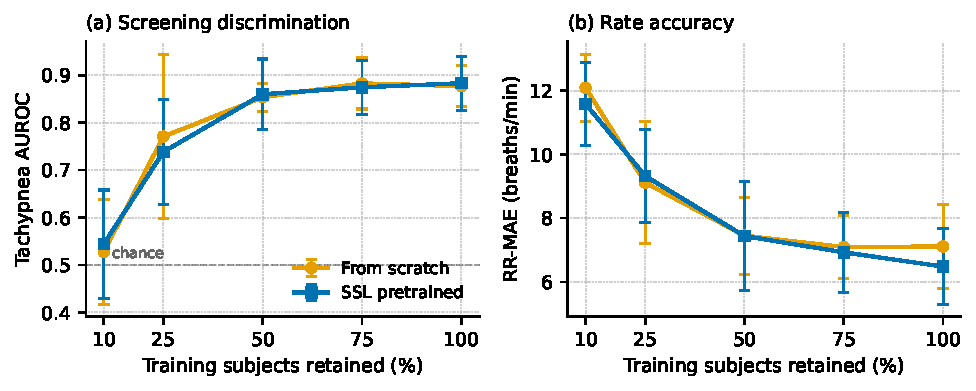
\includegraphics[width=\linewidth]{fig/fig_dataeff.pdf}
\caption{Data efficiency on pediatric-297. PRISM retrained on nested subsets of the training subjects, from
scratch (orange) vs.\ with self-supervised pretraining (blue); per-fold mean$\pm$SD. (a)~Tachypnea AUROC
saturates by ${\sim}50$--$75\%$ of subjects; (b)~SSL lowers RR-MAE at every fraction.}
\label{fig:dataeff}
\end{figure}

\begin{table}[!t]\centering\small
\caption{Data efficiency: pooled tachypnea AUROC and RR-MAE (breaths/min) vs.\ the fraction of training
subjects retained, from scratch and with SSL pretraining (pediatric-297, five folds).}
\label{tab:dataeff}
\setlength{\tabcolsep}{5pt}
\begin{tabular}{@{}lcccc@{}}
\toprule
Train & \multicolumn{2}{c}{AUROC} & \multicolumn{2}{c}{RR-MAE}\\
\cmidrule(lr){2-3}\cmidrule(lr){4-5}
frac. & scratch & SSL & scratch & SSL\\
\midrule
$10\%$  & 0.47 & 0.47 & 12.1 & 11.6\\
$25\%$  & 0.77 & 0.70 & 9.1  & 9.3\\
$50\%$  & 0.84 & 0.85 & 7.5  & 7.4\\
$75\%$  & 0.86 & 0.85 & 7.1  & 6.9\\
$100\%$ & 0.86 & 0.86 & 7.1  & 6.5\\
\bottomrule
\end{tabular}
\end{table}

\subsection{Ablations as Hypotheses, with Paired Confidence Intervals}
Rather than reading raw metric shifts as evidence, we test the ablations as hypotheses under \emph{paired}
subject-bootstrap comparison (Table~\ref{tab:ablh}). \textbf{H1 (representation):} the learned encoder
\emph{as a whole} is decisively load-bearing---raw-flow FFT discriminates tachypnea at AUROC $0.72$, and the
self-supervised spectral-temporal encoder lifts this to $0.87$ ($p<10^{-4}$; main-paper component
isolation)---yet no individual encoder \emph{block} is: removing the spectral features or the scan block
leaves AUROC within noise. \textbf{H2 (objective):} the classification/distributional objective is
load-bearing on a \emph{frozen} encoder ($0.833\to0.880$, DeLong $p=0.026$; main paper). \textbf{H3
(context):} age enters both as a model input and through age-conditional conformal calibration; we did not
isolate it with a dedicated ablation and flag this as a gap. \textbf{H4 (pretraining):} self-supervised
pretraining is \emph{not} individually significant on the full model ($\Delta$AUROC $-0.013$, $p=0.55$); its
benefit is modest and concentrated on RR-MAE and the low-label regime (Sec.~data efficiency) and on the
salience variant ($+0.015$). The decisive point for a small cohort: \emph{every} single-component ablation
has a paired $\Delta$AUROC CI that includes zero, so none is individually ``load-bearing''---which is exactly
why the lean model matches the full one. Discrimination is carried by the encoder-as-a-whole (H1) and the
decision framing (H2), not by any one auxiliary block.

\begin{table}[!t]\centering\small
\caption{Ablations as hypotheses: paired $\Delta$AUROC (full $-$ ablated) with subject-bootstrap $95\%$ CI
and DeLong $p$, corrected pediatric-297. \emph{Every} CI includes zero---no single component is individually
load-bearing.}
\label{tab:ablh}
\setlength{\tabcolsep}{4pt}
\begin{tabular}{@{}lccc@{}}
\toprule
Component removed & Ablated AUROC & $\Delta$AUROC $[95\%$ CI$]$ & DeLong $p$\\
\midrule
Spectral features        & 0.885 & $-0.034\,[-0.071,+0.001]$ & 0.071\\
Scan block               & 0.854 & $-0.003\,[-0.040,+0.032]$ & 0.893\\
Separate trunks          & 0.878 & $-0.026\,[-0.062,+0.006]$ & 0.149\\
Prototype bank           & 0.839 & $+0.012\,[-0.019,+0.044]$ & 0.458\\
Codebook                 & 0.866 & $-0.014\,[-0.051,+0.023]$ & 0.462\\
Heteroscedastic head     & 0.873 & $-0.021\,[-0.051,+0.006]$ & 0.169\\
Self-supervised pretrain & 0.865 & $-0.013\,[-0.057,+0.029]$ & 0.553\\
Modality dropout         & 0.875 & $-0.023\,[-0.055,+0.006]$ & 0.133\\
Lean (proto$+$code$+$het off) & 0.866 & $-0.014\,[-0.047,+0.015]$ & 0.365\\
\midrule
\multicolumn{4}{@{}l}{Full PRISM (reference): AUROC $0.852$, $n{=}297$}\\
\bottomrule
\end{tabular}
\end{table}

%% appendix_selection.tex -- paste-in fragment (\input into prism_breath_supplementary.tex).
%% Sources: scripts/selection_criterion_experiment.py (the A/B), scripts/verify_main_run.py
%% (committed-vs-measured), scripts/identify_baseline_checkpoint.py (which weights the published
%% baselines actually evaluated), scripts/reselect_baseline_checkpoints.py (the matched arm).

\section{Checkpoint Selection Is Part of the Decision Rule}
\label{app:selection}

Section~\ref{sec:selmatrix} reports the selection-rule $\times$ model-family comparison and the
mechanism it establishes. This appendix records the supporting detail: the observational signal that
prompted the audit, the per-fold interventional result, and the provenance of our reported headline.

\subsection{The criterion was misaligned}
Our training loop selected each fold's checkpoint by a validation composite dominated by regression
error, $\text{score} = \text{val MAE} + 5\cdot\text{review rate}$. Across the ten folds of the two full
runs we have, that selected validation MAE correlates \emph{positively} with test tachypnea AUROC
($r={+}0.879$, $p=0.0008$) --- lower validation MAE goes with a \emph{worse} test screen. The effect holds
within each run separately (${+}0.897$, $n{=}5$, $p=0.039$; ${+}0.821$, $n{=}5$, $p=0.088$) and survives
partialling out each fold's RR spread (${+}0.854$, $p=0.0017$); the obvious confound pushes the other way,
since fold RR spread correlates negatively with both quantities.

\subsection{An interventional test}
Correlation across folds is weak evidence, so we ran the intervention. Two complete five-fold runs,
identical in data, folds, architecture, budget and seed, differing \emph{only} in the selection rule
(Table~\ref{tab:selection}):

\begin{table}[!t]
\caption{Checkpoint selection, held-out test performance ($n{=}332$, 84 positive). The two criteria move
the two metrics in opposite directions. Paired DeLong for AUROC; paired Wilcoxon on per-subject absolute
error for MAE.}
\label{tab:selection}\centering\small
\begin{tabular}{@{}lccc@{}}\toprule
 & val-MAE selection & val-AUROC selection & paired test\\\midrule
Tachypnea AUROC   & 0.827 & \textbf{0.850} & ${+}0.023\,[{-}0.013,{+}0.061]$, $p=0.22$\
RR-MAE (br/min)   & \textbf{6.22} & 6.90 & ${+}0.68$, $p=1{\times}10^{-4}$\
Sens / Spec @ WHO & 0.55 / 0.92 & 0.55 / 0.92 & 32 decisions flip, 16 each way\
Folds won (AUROC) & 1 / 5 & \textbf{4 / 5} & ---\\bottomrule
\end{tabular}
\end{table}

Only the MAE cost is significant. The honest summary is therefore not ``selecting on AUROC is better'':
it is that \emph{selecting on regression error reliably buys about $0.7$ breaths/min of RR-MAE and gives
up an amount of decision quality this cohort is too small to resolve}. What makes us take the direction
seriously is where the difference sits. The gain from decision-aware selection is monotone in difficulty,
and largest exactly where the screen is weakest: ${+}0.086$ AUROC in the $<$2mo band ($0.650\to0.736$),
${+}0.027$ at $2$--$12$mo, ${+}0.004$ at $12$--$60$mo. That is the same age gradient the classification
reframing of the main paper shows, and the same one the independent replication shows.

\subsection{Why our headline moved}
This also resolves a discrepancy a reader of our earlier preprint would notice. That draft reported
pooled AUROC $0.881$; the regenerated main run reports $0.827$. The gap is not the age-label correction
($+0.002$), nor extractor leakage ($+0.005$ to $+0.019$), nor the cohort (on the identical 297 subjects
the new run scores $0.826$ where the old scored $0.875$). It is selection variance under a criterion that
does not track the endpoint: honest retrains of this configuration span AUROC $0.83$--$0.89$. We report
the regenerated run, and we no longer regard a single favourable draw under an endpoint-blind criterion
as a reportable operating point.

\subsection{Fairness of the comparison}
The audit behind Section~\ref{sec:selmatrix} established that the published extractors were never
checkpoint-selected: their drivers evaluate whatever weights remain resident when training returns, so
the committed predictions come from the final epoch, and the checkpoint the trainer flags as best is
written but never loaded. We verified this bit-exactly on two folds (maximum
$|\Delta\mathrm{RR}|=0.000$ against the last epoch, versus $9.5$~breaths/min against the flagged
checkpoint). Because every epoch was checkpointed, the matched arm required inference only, and each
model was given the same number of candidate checkpoints so that search budget could not act as a
confound. Harnesses: \texttt{scripts/identify\_baseline\_checkpoint.py},
\texttt{scripts/reselect\_baseline\_checkpoints.py}, \texttt{scripts/selection\_matrix.py}.


\end{document}
